\documentclass[a4paper,12pt,oneside]{book}

%%%%%%%%%%%%%%%%%%%%%%%%%%%%%%%%%%%%%%%%%%%%%%%%%%%%%%%%%%%%%%
%%% Encodage, langue et police
%%%%%%%%%%%%%%%%%%%%%%%%%%%%%%%%%%%%%%%%%%%%%%%%%%%%%%%%%%%%%%
\usepackage[utf8]{inputenc}
\usepackage[T1]{fontenc}
\usepackage{lmodern}
\usepackage[french]{babel}
\usepackage[a4paper,top=2.5cm,bottom=2.5cm,left=2.5cm,right=2.5cm,headheight=15pt]{geometry}
\linespread{1.15}

%%%%%%%%%%%%%%%%%%%%%%%%%%%%%%%%%%%%%%%%%%%%%%%%%%%%%%%%%%%%%%
%%% Paquets
%%%%%%%%%%%%%%%%%%%%%%%%%%%%%%%%%%%%%%%%%%%%%%%%%%%%%%%%%%%%%%
\usepackage{graphicx}
\graphicspath{{images/}}
\usepackage{float}
\usepackage{array,booktabs,tabularx,multirow,colortbl}
\usepackage[table]{xcolor}
\usepackage{enumitem}
\usepackage{amsmath,amssymb}
\usepackage[bottom]{footmisc}
\usepackage{caption}
\captionsetup{font=small,labelfont=bf,labelsep=endash}
\usepackage{listings}
\usepackage[footnote]{acronym}
\usepackage{pgfgantt}
\usepackage{tikz}
\usetikzlibrary{shapes.geometric,shapes.multipart,arrows.meta,positioning,fit,calc,backgrounds}
\usepackage{url}
\usepackage[round]{natbib}
\usepackage{hyperref}
\hypersetup{colorlinks=true,linkcolor=black,citecolor=black,urlcolor=black,
  pdftitle={Transformation numérique des processus analytiques},
  pdfauthor={Nesrine Ferchichi}}

%%%%%%%%%%%%%%%%%%%%%%%%%%%%%%%%%%%%%%%%%%%%%%%%%%%%%%%%%%%%%%
%%% Couleurs et styles communs (tableaux, schémas TikZ)
%%%%%%%%%%%%%%%%%%%%%%%%%%%%%%%%%%%%%%%%%%%%%%%%%%%%%%%%%%%%%%
\definecolor{bleu}{RGB}{31,78,121}
\definecolor{bleuclair}{RGB}{221,235,247}
\definecolor{vert}{RGB}{56,118,29}
\definecolor{orange}{RGB}{191,96,0}
\definecolor{gris}{RGB}{80,80,80}

\newcommand{\entete}[1]{\textcolor{white}{\textbf{#1}}}
\newcommand{\enteteligne}{\rowcolor{bleu}}
\newcolumntype{Y}{>{\raggedright\arraybackslash}X}

\tikzset{
  bloc/.style={draw=bleu, fill=bleuclair, rounded corners=3pt, align=center,
               minimum height=9mm, text width=#1, font=\small},
  bloc/.default=3cm,
  blocvert/.style={bloc=#1, draw=vert, fill=vert!10},
  blocvert/.default=3cm,
  blocorange/.style={bloc=#1, draw=orange, fill=orange!10},
  blocorange/.default=3cm,
  fleche/.style={-{Stealth[length=2.4mm]}, thick, draw=gris},
  doublefleche/.style={{Stealth[length=2.4mm]}-{Stealth[length=2.4mm]}, thick, draw=gris},
  etiq/.style={font=\scriptsize, align=center, text=gris},
  cadre/.style={draw=gris, dashed, rounded corners=4pt, inner sep=3mm},
  decision/.style={diamond, aspect=2.2, draw=orange, fill=orange!10, align=center,
                   font=\small, inner sep=1pt},
  debutfin/.style={rounded rectangle, draw=bleu, fill=bleu, text=white,
                   font=\small\bfseries, minimum height=8mm, minimum width=2.4cm},
  acteur/.style={font=\small, align=center},
  cu/.style={ellipse, draw=bleu, fill=bleuclair, align=center, font=\small,
             minimum height=9mm, text width=3.6cm, inner sep=1pt},
}

% Petit bonhomme UML pour les diagrammes de cas d'utilisation
\newcommand{\bonhomme}[2]{% #1 = position, #2 = nom
  \begin{scope}[shift={#1}, thick, draw=gris]
    \draw (0,0.55) circle (0.18);
    \draw (0,0.37) -- (0,-0.15);
    \draw (-0.3,0.2) -- (0.3,0.2);
    \draw (0,-0.15) -- (-0.22,-0.55);
    \draw (0,-0.15) -- (0.22,-0.55);
    \node[acteur, below] at (0,-0.6) {#2};
  \end{scope}}

\lstset{basicstyle=\ttfamily\footnotesize, breaklines=true, frame=single,
  rulecolor=\color{gris}, backgroundcolor=\color{bleuclair!50},
  keywordstyle=\color{bleu}\bfseries, commentstyle=\color{vert}\itshape,
  showstringspaces=false, columns=fullflexible, keepspaces=true,
  literate={é}{{\'e}}1 {è}{{\`e}}1 {à}{{\`a}}1 {ç}{{\c c}}1 {ê}{{\^e}}1}

%%%%%%%%%%%%%%%%%%%%%%%%%%%%%%%%%%%%%%%%%%%%%%%%%%%%%%%%%%%%%%
%%% Titres, en-têtes et pieds de page
%%%%%%%%%%%%%%%%%%%%%%%%%%%%%%%%%%%%%%%%%%%%%%%%%%%%%%%%%%%%%%
\setcounter{tocdepth}{2}
\setcounter{secnumdepth}{3}

\usepackage{titlesec}
\titleformat{\chapter}[display]
  {\normalfont\huge\bfseries\color{bleu}}{\chaptertitlename\ \thechapter}{16pt}{\Huge}
\titlespacing*{\chapter}{0pt}{-30pt}{30pt}
\titleformat{\section}{\normalfont\Large\bfseries\color{bleu}}{\thesection}{1em}{}
\titleformat{\subsection}{\normalfont\large\bfseries}{\thesubsection}{1em}{}

\usepackage{fancyhdr}
\pagestyle{fancy}
\fancyhf{}
\fancyhead[R]{\bfseries\thepage}
\fancyhead[L]{\small\nouppercase{\leftmark}}
\renewcommand{\headrulewidth}{0.8pt}
\fancypagestyle{plain}{\fancyhf{}\fancyfoot[C]{\thepage}\renewcommand{\headrulewidth}{0pt}}

\setlist{itemsep=2pt, topsep=4pt}
\raggedbottom

%%%%%%%%%%%%%%%%%%%%%%%%%%%%%%%%%%%%%%%%%%%%%%%%%%%%%%%%%%%%%%
\begin{document}
%%%%%%%%%%%%%%%%%%%%%%%%%%%%%%%%%%%%%%%%%%%%%%%%%%%%%%%%%%%%%%

\frontmatter
\begin{titlepage}
\begin{center}

\begin{minipage}[c]{0.2\textwidth}
  
\includegraphics[height=2.3cm]{logo-ensit.png}
\end{minipage}%
\begin{minipage}[c]{0.6\textwidth}
  \centering\small
  République Tunisienne\\
  Ministère de l'Enseignement Supérieur et de la Recherche Scientifique\\[0.15cm]
  \textbf{Université de Tunis}\\
  \textbf{École Nationale Supérieure d'Ingénieurs de Tunis}
\end{minipage}%
\begin{minipage}[c]{0.2\textwidth}
  \raggedleft
\includegraphics[height=2.3cm]{logo-bqube.png}
\end{minipage}

\vspace{1.6cm}

{\Large \textsc{\textbf{Rapport de Projet de Fin d'Études}}}\\[0.3cm]
% À compléter : préciser la spécialité exacte du diplôme
{\large En vue de l'obtention du Diplôme National d'Ingénieur}

\vspace{1cm}
{\color{bleu}\rule{\linewidth}{0.6mm}}\\[0.5cm]
{\LARGE \bfseries Transformation numérique des processus analytiques :\\[0.2cm]
du LIMS aux machines connectées}\\[0.4cm]
{\color{bleu}\rule{\linewidth}{0.6mm}}

\vspace{1.2cm}
{\large Réalisé par :}\\[0.2cm]
{\Large \textbf{Nesrine \textsc{Ferchichi}}}

\vspace{1.4cm}

\begin{tabular}{@{}r@{\hspace{0.5cm}}l@{}}
  \emph{Encadrante universitaire :} & Mme Besma \textsc{Fayech} \\[0.2cm]
  \emph{Encadrants entreprise :}    & M. Mohamed \textsc{Saidi} \\
                                    & M. Hazem \textsc{Manai} \\[0.4cm]
  \emph{Président(e) du jury :}     & \makebox[5.5cm]{\dotfill} \\[0.2cm]
  \emph{Rapporteur(e) :}            & \makebox[5.5cm]{\dotfill} \\
\end{tabular}

\vfill
{\small Projet réalisé au sein de \textbf{BQube ITs}}\\[0.3cm]
{\color{bleu}\rule{45mm}{0.4pt}}\\[0.2cm]
{\large Année universitaire 2025--2026}

\end{center}
\end{titlepage}

\thispagestyle{empty}
\begin{center}
{\Large\bfseries Appréciations et signature de l'encadrante universitaire}\\[0.5cm]
\fbox{\begin{minipage}[t][8.5cm]{14cm}\hfill\end{minipage}}

\vspace{1cm}
{\Large\bfseries Appréciations et signature des encadrants entreprise}\\[0.5cm]
\fbox{\begin{minipage}[t][8.5cm]{14cm}\hfill\end{minipage}}
\end{center}
\clearpage

\chapter*{Remerciements}
\thispagestyle{plain}

Au terme de ce projet de fin d'études, je tiens à exprimer ma profonde gratitude à toutes les personnes qui ont contribué, de près ou de loin, à la réalisation de ce travail.

J'exprime ma profonde reconnaissance à Madame Besma \textsc{Fayech}, mon encadrante universitaire, pour son accompagnement, sa disponibilité et ses précieux conseils tout au long de ce projet. Je la remercie sincèrement pour la confiance qu'elle m'a accordée, pour son écoute et pour ses orientations, qui m'ont permis de progresser, d'enrichir mes connaissances et de mener à bien les différentes étapes de ce travail.

Je remercie également toute l'équipe de BQube ITs de m'avoir offert l'opportunité de réaliser mon projet de fin d'études au sein de l'entreprise. Je la remercie pour son accueil, sa confiance, sa disponibilité, ainsi que pour l'environnement professionnel et enrichissant dans lequel j'ai pu évoluer.

J'adresse un remerciement particulier à M. Mohamed \textsc{Saidi}, M. Hazem \textsc{Manai}, M. Omar \textsc{Trabelsi} et Mme Eya \textsc{Ben Della} pour leur encadrement, leur disponibilité, leurs précieux conseils et leur accompagnement tout au long de ce projet.

Je remercie aussi les équipes du Centre Technique de l'Agro-Alimentaire et des Laboratoires Pharmaghreb pour leur accueil et leur collaboration.

Je remercie les membres du jury d'avoir accepté d'évaluer ce travail, ainsi que l'ensemble des enseignants de l'École Nationale Supérieure d'Ingénieurs de Tunis pour la qualité de la formation reçue.

Enfin, je tiens à remercier mon partenaire pour sa présence, son soutien, sa compréhension et ses encouragements. À mon très cher père, qui a toujours été à mes côtés pour me soutenir et m'encourager : ta bienveillance et ta présence m'ont donné la force d'affronter les obstacles. À ma très chère mère : rien de ce que je pourrais faire ou dire ne saurait te remercier comme il se doit ; que ce travail soit le témoignage de ma profonde reconnaissance. À mes chers frères, pour leurs conseils, leurs encouragements et leur soutien constant tout au long de mes études : que Dieu les protège et leur offre chance et bonheur.


\tableofcontents
\listoffigures
\listoftables

\chapter*{Liste des sigles et acronymes}
\addcontentsline{toc}{chapter}{Liste des sigles et acronymes}
\markboth{Liste des sigles et acronymes}{}
\begin{acronym}[ISO/CEI 17025]
  \acro{AJAX}{\emph{Asynchronous JavaScript and XML}}
  \acro{BPF}{Bonnes Pratiques de Fabrication}
  \acro{CTAA}{Centre Technique de l'Agro-Alimentaire}
  \acro{DLC}{Date Limite de Consommation}
  \acro{FTP}{\emph{File Transfer Protocol}}
  \acro{HTML}{\emph{HyperText Markup Language}}
  \acro{HTTP}{\emph{HyperText Transfer Protocol}}
  \acro{I2C}[I$^2$C]{\emph{Inter-Integrated Circuit}}
  \acro{IHM}{Interface Homme-Machine}
  \acro{IIoT}{\emph{Industrial Internet of Things}}
  \acro{IoT}{\emph{Internet of Things}}
  \acro{IP}{\emph{Internet Protocol}}
  \acro{ISO/CEI 17025}{Norme relative aux exigences générales concernant la compétence des laboratoires d'étalonnages et d'essais}
  \acro{JSON}{\emph{JavaScript Object Notation}}
  \acro{LCD}{\emph{Liquid Crystal Display}}
  \acro{LIMS}{\emph{Laboratory Information Management System}}
  \acro{M2M}{\emph{Machine-to-Machine}}
  \acro{MES}{\emph{Manufacturing Execution System}}
  \acro{MT-SICS}{\emph{Mettler Toledo Standard Interface Command Set}}
  \acro{NFC}{\emph{Near Field Communication}}
  \acro{OGM}{Organisme Génétiquement Modifié}
  \acro{PHP}{\emph{PHP: Hypertext Preprocessor}}
  \acro{QR}{\emph{Quick Response} (code)}
  \acro{ROI}{\emph{Return On Investment} (retour sur investissement)}
  \acro{RS-232}{\emph{Recommended Standard 232}}
  \acro{SQL}{\emph{Structured Query Language}}
  \acro{TCP}{\emph{Transmission Control Protocol}}
  \acro{TND}{Dinar tunisien}
  \acro{UART}{\emph{Universal Asynchronous Receiver-Transmitter}}
  \acro{UML}{\emph{Unified Modeling Language}}
  \acro{Wi-Fi}{\emph{Wireless Fidelity}}
  \acro{XML}{\emph{eXtensible Markup Language}}
\end{acronym}

\mainmatter
\chapter*{Introduction générale}
\addcontentsline{toc}{chapter}{Introduction générale}
\markboth{Introduction générale}{}

À l'ère de la transformation numérique, l'Industrie~4.0 marque une évolution majeure des secteurs industriels et des laboratoires. Elle repose sur l'intégration des technologies numériques, de l'Internet des objets (\ac{IoT}), des systèmes d'information et de l'automatisation des processus \citep{kagermann2013,lasi2014}. Cette transformation améliore la performance opérationnelle, renforce la qualité des produits et des analyses, assure une traçabilité complète des opérations et facilite la prise de décision grâce à l'exploitation des données en temps réel.

Les laboratoires d'analyses sont directement concernés. Soumis à des exigences strictes de fiabilité et de traçabilité, notamment celles de la norme \ac{ISO/CEI 17025} \citep{iso17025}, ils produisent chaque jour un grand volume de données : demandes, échantillons, mesures, résultats et rapports. Lorsque ces données sont saisies à la main et dispersées sur plusieurs supports, les risques d'erreur augmentent, les délais s'allongent et la reconstitution de l'historique devient difficile.

C'est dans ce contexte que s'inscrit ce projet de fin d'études, réalisé au sein de BQube ITs, entreprise tunisienne spécialisée dans les solutions numériques pour l'industrie et les laboratoires, en particulier les systèmes \ac{MES} et \ac{LIMS}. Le projet comporte deux volets complémentaires qui couvrent les deux niveaux de la transformation numérique d'un laboratoire :
\begin{itemize}
  \item \textbf{le niveau du système d'information}, au Centre Technique de l'Agro-Alimentaire (\ac{CTAA}) : participation au déploiement d'un \ac{LIMS} (paramétrage, étiquetage par codes-barres et codes \ac{QR}, formation des utilisateurs), puis conception et développement d'un module de traçabilité ;
  \item \textbf{le niveau des équipements}, aux Laboratoires Pharmaghreb : étude de la connectivité de dix équipements de laboratoire, puis conception, réalisation et test d'un prototype d'acquisition qui récupère automatiquement les mesures d'une balance par liaison \ac{RS-232} et les transmet par \ac{Wi-Fi}. Ce prototype est fonctionnel et attend son déploiement.
\end{itemize}

La problématique générale peut se formuler ainsi : \emph{comment digitaliser les processus analytiques d'un laboratoire, de la gestion des échantillons jusqu'aux machines connectées, tout en garantissant la fiabilité et la traçabilité des données ?}

Ce rapport s'organise en quatre chapitres :
\begin{itemize}
  \item le \textbf{premier chapitre} présente le cadre général du projet : l'entreprise d'accueil, les deux cas d'étude, l'analyse de l'existant, la problématique, la méthodologie et la planification ;
  \item le \textbf{deuxième chapitre} est consacré à l'analyse et à la spécification des besoins ;
  \item le \textbf{troisième chapitre} détaille la conception du module de traçabilité et du prototype de machine connectée ;
  \item le \textbf{quatrième chapitre} décrit la réalisation : environnement de travail, déploiement du \ac{LIMS}, interfaces développées, tests, formation des utilisateurs et réalisation du prototype.
\end{itemize}
Une conclusion générale dresse le bilan du travail et ouvre des perspectives. L'annexe~\ref{annexe:gains} détaille la méthode d'estimation des gains économiques.

\chapter{Cadre général du projet et démarche de résolution}
\label{chap:cadre-general}

Ce premier chapitre pose les bases du projet. Il présente le contexte professionnel du stage, décrit les deux missions confiées et justifie la démarche retenue pour les mener à bien. Nous présentons d'abord BQube ITs, l'entreprise d'accueil, puis les deux cas d'étude : le déploiement d'un \ac{LIMS} au \ac{CTAA} et la connexion des équipements de laboratoire de Pharmaghreb. Pour chacun, nous analysons l'existant et exposons la solution proposée. Nous formulons ensuite la problématique et les objectifs, avant de présenter la méthodologie et la planification du projet.

%-------------------------------------------------------------
\section{Présentation de l'entreprise d'accueil}
%-------------------------------------------------------------

Le stage s'est déroulé au sein de BQube ITs, société tunisienne de conseil et de services informatiques créée en 2017. Elle conçoit des solutions numériques destinées à l'Industrie~4.0 et accompagne les industriels et les laboratoires dans la digitalisation de leurs processus. Son savoir-faire couvre principalement :
\begin{itemize}
    \item les systèmes \ac{MES}, dédiés au pilotage de la production ;
    \item les systèmes \ac{LIMS}, dédiés à la gestion des laboratoires \citep{gibbon1996} ;
    \item le développement de logiciels sur mesure ;
    \item la numérisation des processus métier.
\end{itemize}
Ses interventions visent à renforcer, chez ses clients, la traçabilité, l'automatisation, la qualité et la gestion des données.

\begin{figure}[H]
  \centering
  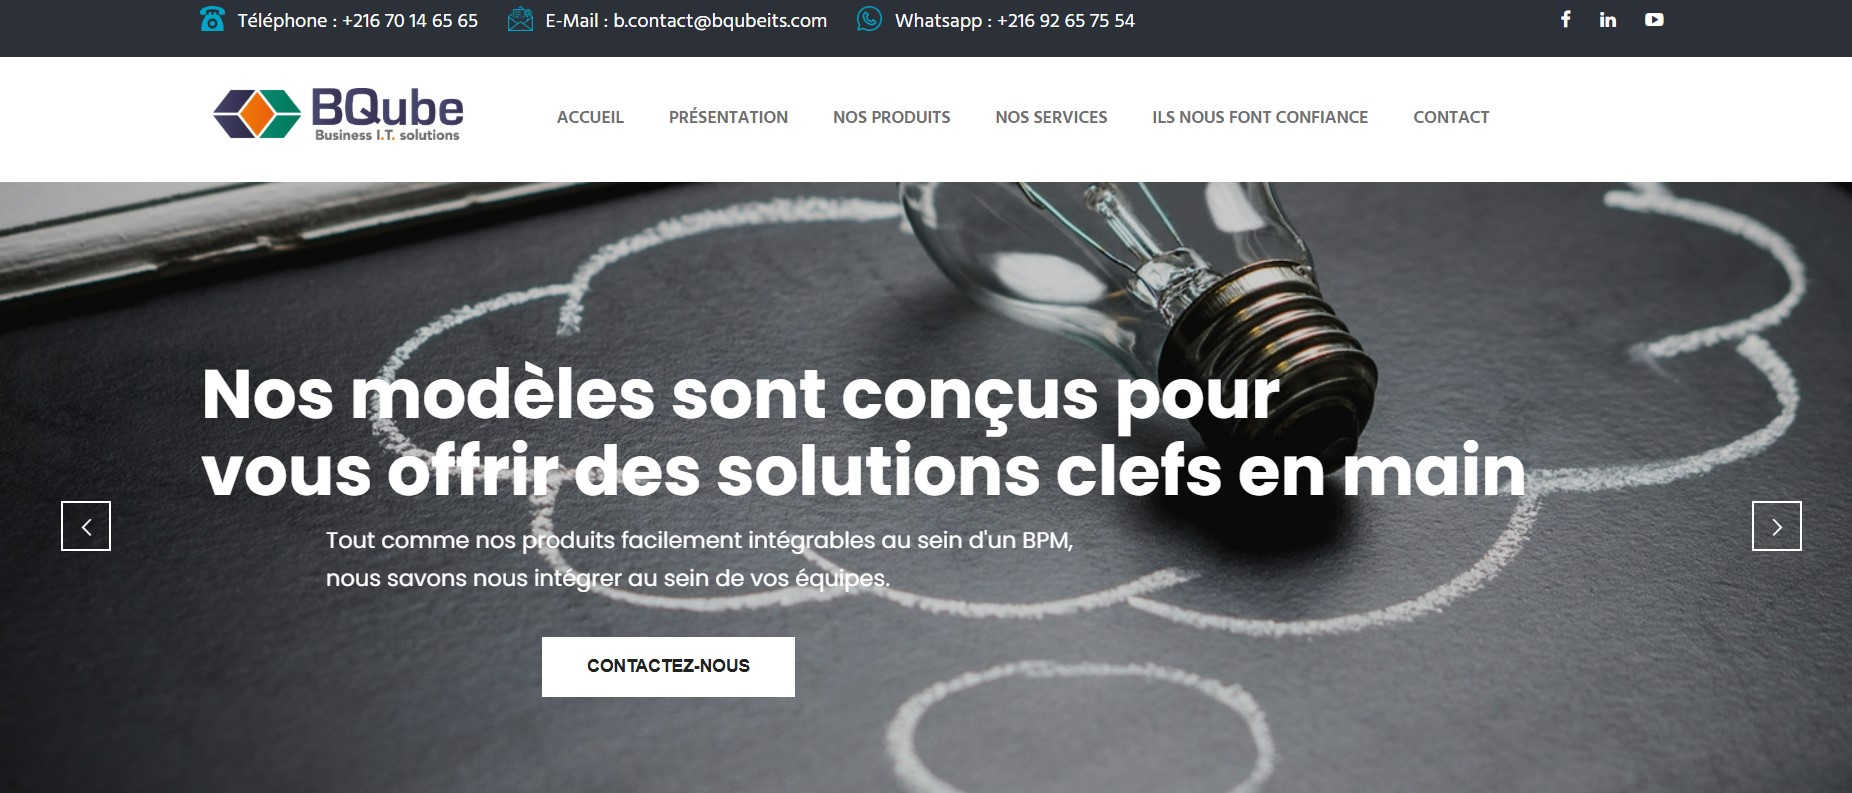
\includegraphics[width=0.45\textwidth]{logo-bqube-grand.jpg}
  \caption{Logo de la société BQube ITs.}
  \label{fig:bqube}
\end{figure}

Le projet de fin d'études s'inscrit dans cette activité à travers deux missions :
\begin{itemize}
    \item \textbf{\ac{CTAA}} : mise en place d'un \ac{LIMS} et développement d'un module de traçabilité dans un centre spécialisé dans l'analyse, le contrôle qualité et l'expertise des produits agroalimentaires ;
    \item \textbf{Pharmaghreb} : étude de la connectivité des équipements de laboratoire d'un industriel pharmaceutique, puis conception et réalisation d'un prototype d'acquisition automatique des mesures.
\end{itemize}

%-------------------------------------------------------------
\section{Premier cas d'étude : le CTAA}
%-------------------------------------------------------------

\subsection{Présentation du cas}

Le \ac{CTAA} est un organisme public tunisien fondé en 1996 \citep{ctaaweb}. Il soutient les industriels du secteur agroalimentaire par de l'assistance technique, de la formation, de la recherche et des analyses de laboratoire accréditées (microbiologie, physico-chimie, analyse sensorielle, recherche d'\ac{OGM}). Sa clientèle se compose :
\begin{itemize}
    \item des entreprises des industries alimentaires ;
    \item des opérateurs commerciaux, importateurs et exportateurs de produits alimentaires ;
    \item des organisations professionnelles, telles que la Fédération nationale de l'agroalimentaire et les chambres syndicales ;
    \item des organismes publics, principalement rattachés aux ministères chargés de l'Industrie, du Commerce, de l'Agriculture et de la Santé.
\end{itemize}

\begin{figure}[H]
  \centering
  
\includegraphics[width=0.28\textwidth]{logo-ctaa.jpg}
  \caption{Logo du Centre Technique de l'Agro-Alimentaire.}
  \label{fig:ctaa}
\end{figure}

Le laboratoire réalise des analyses physico-chimiques, microbiologiques et nutritionnelles, ce qui produit un volume important d'informations à gérer. Le traitement d'un échantillon suit un parcours en quatre étapes :
\begin{enumerate}
    \item la réception de l'échantillon et l'enregistrement de la demande ;
    \item la réalisation des analyses ;
    \item la saisie et la validation des résultats ;
    \item l'édition des rapports d'analyse.
\end{enumerate}
Chaque étape génère des données qui doivent être enregistrées, conservées et accessibles à tout moment.

Le \ac{CTAA} évolue en outre dans un cadre très exigeant en matière de qualité et de traçabilité. La norme \ac{ISO/CEI 17025}, référence internationale applicable aux laboratoires d'essais et d'étalonnage, impose au laboratoire de démontrer sa compétence et de maîtriser toutes les activités susceptibles d'influencer la validité de ses résultats \citep{iso17025}. L'enjeu principal est donc de centraliser et de structurer les informations tout en les rendant accessibles de manière sécurisée.

\subsection{Analyse de l'existant}

L'analyse de l'existant s'appuie sur des observations menées dans le laboratoire et sur des échanges avec ses utilisateurs. Elle a mis en évidence plusieurs contraintes dans la gestion des demandes, des échantillons, des analyses et des informations associées.

\subsubsection*{Volume d'activité}

Le \ac{CTAA} reçoit chaque jour entre 10 et 20 demandes d'analyses, réparties en trois catégories : les demandes d'importation, les demandes d'exportation et les demandes d'autocontrôle. Une demande porte en général sur 1 à 10 échantillons, et chaque échantillon peut nécessiter des analyses physico-chimiques, microbiologiques, ou les deux. Plusieurs intervenants doivent donc enregistrer, consulter et suivre un grand nombre de données tout au long du processus.

\subsubsection*{Identification des échantillons et limites du code-barres}

Avant le projet, les échantillons étaient identifiés par des étiquettes à code-barres linéaire (figure~\ref{fig:codebarre}). Ce mode d'identification présente plusieurs limites :
\begin{itemize}
    \item \textbf{une capacité de stockage réduite} : un code linéaire ne contient qu'une faible quantité d'informations \citep{iso15417} ;
    \item \textbf{une lecture directionnelle} : le code doit être orienté face au lecteur, ce qui ralentit l'opération ;
    \item \textbf{une sensibilité à l'impression} : une étiquette mal imprimée, abîmée ou partiellement masquée peut empêcher la lecture ;
    \item \textbf{un espace d'étiquetage limité} : les désignations longues s'affichent parfois de façon tronquée.
\end{itemize}

\begin{figure}[H]
  \centering
  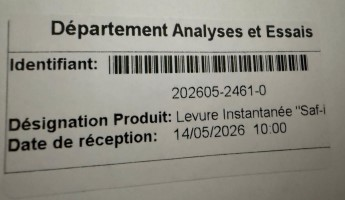
\includegraphics[width=0.42\textwidth]{etiquette-code-barres.jpg}
  \caption{Étiquette d'échantillon à code-barres utilisée avant le projet.}
  \label{fig:codebarre}
\end{figure}

\subsubsection*{Manque de centralisation et de sécurisation des données}

L'usage de plusieurs outils non intégrés entraînait une dispersion des données, des risques d'erreur lors des saisies et des difficultés pour retrouver l'information. Or la norme \ac{ISO/CEI 17025} exige de maîtriser, de tracer et de conserver correctement les informations afin d'assurer la fiabilité des résultats.

\subsubsection*{Traçabilité incomplète des opérations}

Dans un laboratoire accrédité, chaque étape du traitement d'un échantillon doit pouvoir être reconstituée, de sa réception jusqu'à la validation du résultat. L'absence de système intégré limitait la visibilité sur l'utilisateur ayant réalisé chaque opération, sur les étapes de traitement, sur l'historique des modifications et sur les équipements, réactifs et consommables utilisés.

\subsubsection*{Suivi des équipements et des compétences du personnel}

Le laboratoire doit identifier chacun de ses équipements, suivre sa maintenance et son étalonnage, et vérifier régulièrement les compétences et les habilitations de ses agents. Gérées à la main, ces informations rendent plus difficile le respect des échéances.

\subsubsection*{Délais de traitement et absence de suivi en temps réel}

La saisie sur papier et l'attente de la validation et de la signature du responsable allongeaient les délais, en particulier en période de forte activité. Faute de suivi centralisé, un client pouvait devoir revenir au \ac{CTAA} sans connaître l'état exact de sa demande.

\subsubsection*{Synthèse des problèmes identifiés}

Le tableau~\ref{tab:synthese-ctaa} résume les principaux constats et leurs conséquences.

\begin{table}[H]
\centering
\renewcommand{\arraystretch}{1.3}
\begin{tabularx}{\textwidth}{|p{5cm}|Y|}
\hline
\enteteligne \entete{Problème constaté} & \entete{Conséquence} \\ \hline
Identification par code-barres linéaire & Lecture lente ou impossible, informations tronquées \\ \hline
Données dispersées & Erreurs de saisie, recherche d'informations longue \\ \hline
Traçabilité incomplète & Historique difficile à reconstituer lors d'un audit \\ \hline
Suivi manuel des équipements et des habilitations & Échéances de maintenance, d'étalonnage et d'habilitation plus difficiles à tenir \\ \hline
Opérations manuelles et validations papier & Délais allongés, surtout en période de forte activité \\ \hline
Absence de suivi en temps réel & Déplacements et attentes inutiles pour les clients \\ \hline
\end{tabularx}
\caption{Synthèse des problèmes de l'existant au CTAA.}
\label{tab:synthese-ctaa}
\end{table}

\subsubsection*{Analyse des gaspillages selon les sept Muda}

La démarche Lean classe les pertes de temps et de ressources en sept catégories de gaspillage, appelées \emph{Muda} \citep{ohno1988,womack1996}. La figure~\ref{fig:muda} les applique au fonctionnement observé au \ac{CTAA}. Quatre d'entre elles ressortent nettement :
\begin{itemize}
    \item \textbf{l'attente} : délais de validation, de signature et de disponibilité des résultats ;
    \item \textbf{les mouvements inutiles} : clients obligés de revenir pour s'informer de l'état de leur demande ;
    \item \textbf{le surtraitement} : ressaisies et tâches répétitives à faible valeur ajoutée ;
    \item \textbf{les défauts} : erreurs de saisie qu'il faut ensuite détecter et corriger.
\end{itemize}

\begin{figure}[H]
  \centering
  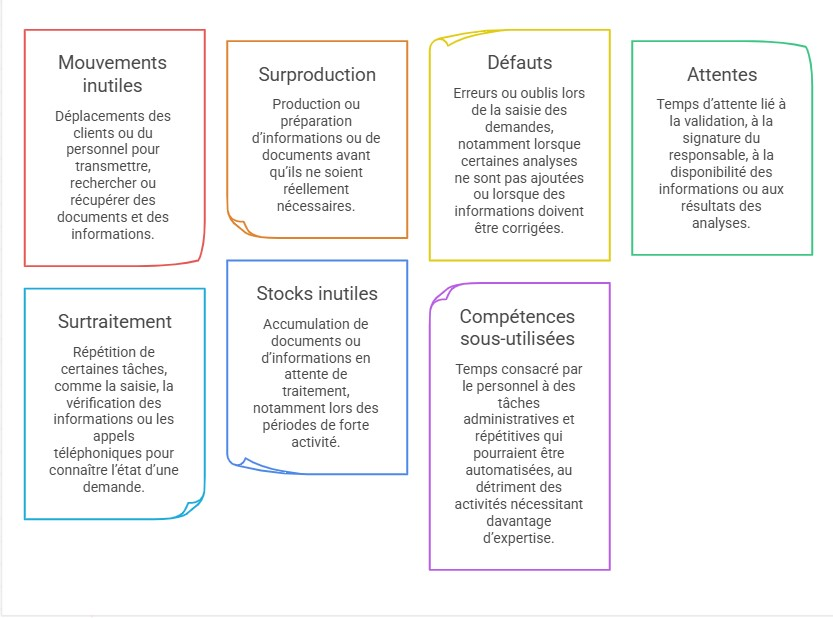
\includegraphics[width=0.85\textwidth]{muda-ctaa.jpg}
  \caption{Les sept Muda appliqués au fonctionnement du CTAA.}
  \label{fig:muda}
\end{figure}

Ces constats confirment la nécessité d'automatiser et de centraliser les processus afin de réduire les tâches à faible valeur ajoutée et d'accélérer le traitement des demandes.

\subsection{Solution proposée}

La solution proposée s'inscrit dans la transformation numérique du laboratoire, que l'on désigne souvent par le terme de « Laboratoire~4.0 ». Le déploiement d'un \ac{LIMS} en constitue l'élément central. Ce système permet de digitaliser et de centraliser les flux analytiques, de structurer les données du laboratoire et de suivre le cycle de vie de chaque échantillon, de sa réception jusqu'à l'émission du résultat validé. Il est complété par :
\begin{itemize}
    \item \textbf{une identification des échantillons par code \ac{QR}} dans le module de gestion des demandes : le code \ac{QR} contient davantage d'informations, se lit dans toutes les orientations et tolère une dégradation partielle de l'étiquette \citep{iso18004}. Les autres modules (réceptions, préparations, stocks) conservent pour l'instant le code-barres, dont la généralisation vers le code \ac{QR} constitue une perspective ;
    \item \textbf{un module de traçabilité} qui, à partir de la lecture d'un code ou de la saisie d'un numéro de série, reconstitue l'historique des opérations associées ;
    \item \textbf{le portail client} du \ac{CTAA}, qui permet aux clients de déposer leurs demandes et de consulter leurs rapports à distance.
\end{itemize}

Le tableau~\ref{tab:comparatif-lims} compare le fonctionnement du laboratoire avant et après le déploiement du \ac{LIMS}.

\begin{table}[H]
\centering
\renewcommand{\arraystretch}{1.25}
\begin{tabularx}{\textwidth}{|p{3.4cm}|Y|Y|}
\hline
\enteteligne \entete{Critère} & \entete{Avant le LIMS} & \entete{Après le LIMS} \\ \hline
Gestion des échantillons & Documents papier, gestion manuelle & Gestion numérique et centralisée \\ \hline
Identification & Code-barres linéaire, saisies manuelles & Code QR pour les échantillons, lecture par douchette \\ \hline
Saisie des données & Ressaisies, risque d'erreur élevé & Saisie unique, contrôles automatiques \\ \hline
Traçabilité & Limitée et dispersée & Historique numérique des opérations \\ \hline
Recherche d'information & Consultation successive de plusieurs documents & Recherche ou scan d'un identifiant \\ \hline
Suivi des demandes & Déplacements ou appels des clients & Suivi en ligne via le portail client \\ \hline
Équipements et habilitations & Suivi manuel des échéances & Suivi centralisé de la métrologie et des habilitations \\ \hline
Sécurité des données & Risque de perte ou de modification & Droits d'accès par rôle et historisation \\ \hline
Prise de décision & Informations peu disponibles & Données centralisées et exploitables \\ \hline
\end{tabularx}
\caption{Comparaison du fonctionnement du CTAA avant et après le déploiement du LIMS.}
\label{tab:comparatif-lims}
\end{table}

\subsubsection*{Évaluation du retour sur investissement}

Les gains économiques ont été estimés selon une méthode en quatre temps, détaillée dans l'annexe~\ref{annexe:gains} : identification des sources de gain, quantification des volumes, estimation du temps gagné par opération, puis valorisation au coût horaire chargé. Deux scénarios encadrent l'incertitude : un scénario \emph{prudent} et un scénario \emph{optimiste}. Le tableau~\ref{tab:gains-ctaa} présente le résultat.

\begin{table}[H]
\centering
\renewcommand{\arraystretch}{1.25}
\begin{tabularx}{\textwidth}{|p{3.6cm}|Y|r|r|}
\hline
\enteteligne \entete{Source de gain} & \entete{Description} & \entete{Prudent} & \entete{Optimiste} \\ \hline
Traitement des demandes & Moins de saisie et de gestion manuelle des demandes & 18\,750 & 25\,000 \\ \hline
Recherche des échantillons & Localisation et identification plus rapides & 22\,500 & 22\,500 \\ \hline
Archivage & Moins de classement et de stockage physique & 3\,000 & 3\,000 \\ \hline
Réduction des erreurs & Moins d'erreurs de saisie et de transcription & 1\,500 & 1\,500 \\ \hline
Consommation de papier & Dématérialisation des documents & 1\,200 & 1\,200 \\ \hline
\rowcolor{bleuclair} \multicolumn{2}{|l|}{\textbf{Gain total annuel estimé (TND/an)}} & \textbf{46\,950} & \textbf{53\,200} \\ \hline
\end{tabularx}
\caption{CTAA : estimation des gains économiques annuels (en TND/an).}
\label{tab:gains-ctaa}
\end{table}

À partir de ces gains et d'un investissement initial de 60\,000~\ac{TND}, nous calculons deux indicateurs. Le \textbf{délai de récupération} (en mois) et le \textbf{\ac{ROI} sur trois ans} sont donnés par :
\[
\text{Délai} = \frac{I_0}{G_{\text{an}}} \times 12
\qquad\qquad
\text{ROI}_{3\,\text{ans}} = \frac{3\,G_{\text{an}} - I_0}{I_0} \times 100
\]
où $I_0$ est l'investissement initial et $G_{\text{an}}$ le gain annuel. Nous retenons un horizon de trois ans, car un \ac{LIMS} est un investissement durable dont les gains s'étalent sur plusieurs années. Le calcul suppose qu'aucun coût récurrent supplémentaire n'est ajouté ; l'annexe~\ref{annexe:gains} étudie la sensibilité du résultat à ce paramètre.

\begin{table}[H]
\centering
\renewcommand{\arraystretch}{1.25}
\begin{tabular}{|l|r|r|}
\hline
\enteteligne \entete{Indicateur} & \entete{Scénario prudent} & \entete{Scénario optimiste} \\ \hline
Gain annuel & 46\,950~TND & 53\,200~TND \\ \hline
Investissement initial & 60\,000~TND & 60\,000~TND \\ \hline
Délai de récupération & 15,3 mois & 13,5 mois \\ \hline
ROI sur 3 ans & 134,75\,\% & 166\,\% \\ \hline
\end{tabular}
\caption{Délai de récupération et ROI de la solution au CTAA.}
\label{tab:roi-ctaa}
\end{table}

Le délai de récupération dépasse légèrement un an : la première année ne suffit pas à rentabiliser l'investissement, mais celui-ci est largement amorti sur trois ans. Au-delà de ces gains chiffrables, le \ac{LIMS} apporte des bénéfices qualitatifs importants : meilleure traçabilité des échantillons et des analyses, données plus fiables, risque réduit de perte d'information et respect facilité des exigences de la norme \ac{ISO/CEI 17025}.

%-------------------------------------------------------------
\section{Deuxième cas d'étude : Pharmaghreb}
%-------------------------------------------------------------

\subsection{Présentation du cas}

Les Laboratoires Pharmaghreb ont été fondés en 1985 par M. Radhouane Bouzguenda, pharmacien, et se présentent comme la première industrie pharmaceutique privée de Tunisie \citep{pharmaghrebweb}. L'entreprise fabrique des médicaments et des produits parapharmaceutiques, produit sous licence et noue des partenariats industriels. Elle s'est étendue en Algérie en 2011 avec la création des laboratoires Pharmidal NS, et a obtenu en 2019 les certifications ISO~9001 (management de la qualité) et ISO~14001 (management environnemental). La qualité et la sécurité sont au cœur de son activité : elle applique les \ac{BPF} et assure la pharmacovigilance, c'est-à-dire la collecte, le suivi et l'évaluation des effets indésirables de ses médicaments.

\begin{figure}[H]
  \centering
  
\includegraphics[width=0.45\textwidth]{logo-pharmaghreb.jpg}
  \caption{Logo des Laboratoires Pharmaghreb.}
  \label{fig:pharmaghreb}
\end{figure}

Une industrie pharmaceutique enchaîne plusieurs étapes : fabrication, conditionnement, contrôle qualité, puis stockage avant distribution. Ses laboratoires de contrôle vérifient les caractéristiques des matières premières et des produits à chaque étape, à l'aide d'équipements de mesure de précision : balances analytiques, pH-mètres, titrateurs, polarimètres, spectromètres, etc. Notre étude a porté sur dix de ces équipements, principalement de marque Mettler Toledo ; leur liste et le résultat de leur étude figurent au chapitre~\ref{chap:realisation} (tableau~\ref{tab:etude-equipements}).

\subsection{Analyse de l'existant}

Ces équipements disposent de plusieurs interfaces de communication (\ac{RS-232}, Ethernet, USB), mais celles-ci ne sont pas exploitées : aucune solution ne transfère les mesures vers un système informatique centralisé. L'étude met en évidence les difficultés suivantes.

\subsubsection*{Difficultés liées aux mesures}
\begin{itemize}
    \item \textbf{Saisie manuelle des résultats} : l'opérateur lit la valeur sur l'équipement puis la recopie, ce qui provoque des erreurs de transcription et allonge le traitement.
    \item \textbf{Intégration limitée au système d'information} : les mesures restent sur l'équipement ou sont enregistrées à part, ce qui complique leur centralisation.
    \item \textbf{Traçabilité fragile} : sans association automatique entre la mesure, l'équipement, l'opérateur et l'horodatage, la reconstitution de l'historique est difficile, alors que les \ac{BPF} exigent l'intégrité des données de contrôle.
    \item \textbf{Exploitation limitée des données} : la dispersion des mesures complique leur consultation, leur archivage et leur réutilisation.
\end{itemize}

\subsubsection*{Difficultés liées à l'état des équipements}
\begin{itemize}
    \item \textbf{Visibilité limitée} : sans suivi en temps réel, l'état de fonctionnement des équipements est difficile à connaître.
    \item \textbf{Anticipation limitée des pannes} : sans suivi continu, les anomalies sont détectées tardivement et la maintenance est moins bien planifiée.
\end{itemize}

\subsection{Solution proposée}

Nous avons proposé une démarche de \emph{rétrofit} numérique inspirée de l'Industrie~4.0 \citep{lee2015} : plutôt que de remplacer les équipements, nous leur ajoutons des capacités de communication afin que leurs mesures soient collectées et transmises automatiquement aux systèmes numériques. La démarche comporte deux étapes :
\begin{enumerate}
    \item \textbf{l'étude de connectivité} de chaque équipement : interfaces disponibles, protocoles supportés (\ac{MT-SICS}, \ac{TCP}/\ac{IP}, \ac{FTP}) et tests de communication ;
    \item \textbf{la conception et la réalisation d'un module d'acquisition} pour les équipements qui ne disposent que d'une liaison série : un boîtier fondé sur un microcontrôleur ESP8266 récupère les mesures d'une balance par \ac{RS-232}, identifie l'opérateur par badge \ac{NFC} et transmet les données par \ac{Wi-Fi}.
\end{enumerate}

À terme, la collecte continue des données prépare la \emph{maintenance prédictive}, qui repose sur la surveillance des paramètres de fonctionnement et l'analyse de leur historique pour détecter les signes précurseurs de défaillance \citep{mobley2002}.

\textbf{Périmètre de la mission.} L'étude de connectivité a été menée sur dix équipements. Le module d'acquisition a été conçu, réalisé et testé avec succès sur une balance Mettler Toledo XSR205 : il s'agit d'un \textbf{prototype complet et fonctionnel, en attente de déploiement} sur site. Son intégration au système d'information et la connexion des autres équipements constituent les perspectives du projet.

\subsubsection*{Estimation des gains économiques annuels}

Les gains attendus ont été estimés avec la même méthode que pour le \ac{CTAA} (annexe~\ref{annexe:gains}). Ils proviennent de la suppression des saisies manuelles, de la baisse des erreurs, de la centralisation des données et de l'amélioration de la disponibilité des équipements (tableau~\ref{tab:gains-pharmaghreb}). Il s'agit d'une \textbf{approximation} : le coût de déploiement n'étant pas encore arrêté, le \ac{ROI} réel sera calculé lors du déploiement.

\begin{table}[H]
\centering
\renewcommand{\arraystretch}{1.25}
\begin{tabularx}{\textwidth}{|p{3.8cm}|Y|r|r|}
\hline
\enteteligne \entete{Source de gain} & \entete{Description} & \entete{Prudent} & \entete{Optimiste} \\ \hline
Réduction des saisies manuelles & Moins de temps consacré à la recopie des mesures & 12\,000 & 15\,000 \\ \hline
Réduction du temps de collecte & Acquisition automatique des données & 10\,000 & 12\,500 \\ \hline
Disponibilité des équipements & Détection plus précoce des anomalies & 7\,500 & 7\,500 \\ \hline
Centralisation des données & Moins de recherche et de consolidation & 5\,000 & 5\,000 \\ \hline
Réduction des erreurs de saisie & Moins d'erreurs de transcription & 2\,000 & 2\,000 \\ \hline
\rowcolor{bleuclair} \multicolumn{2}{|l|}{\textbf{Gain total annuel estimé (TND/an)}} & \textbf{36\,500} & \textbf{42\,000} \\ \hline
\end{tabularx}
\caption{Pharmaghreb : estimation approximative des gains économiques annuels (en TND/an).}
\label{tab:gains-pharmaghreb}
\end{table}

%-------------------------------------------------------------
\section{Problématique et objectifs}
%-------------------------------------------------------------

Les deux cas d'étude révèlent un constat commun : dans les laboratoires, la saisie manuelle, la dispersion des données et le manque de suivi pénalisent la fiabilité, la rapidité et la traçabilité des résultats. La problématique générale du projet se formule ainsi :

\begin{quote}
\emph{Comment digitaliser les processus analytiques d'un laboratoire, de la gestion des échantillons jusqu'aux machines connectées, tout en garantissant la fiabilité et la traçabilité des données ?}
\end{quote}

Elle se décline en deux questions, une par cas d'étude :
\begin{itemize}
    \item \textbf{\ac{CTAA}} : comment centraliser la gestion des échantillons et garantir leur traçabilité grâce à un \ac{LIMS} et à un module dédié ?
    \item \textbf{Pharmaghreb} : comment connecter des équipements d'analyse existants au système d'information afin d'automatiser la remontée des mesures ?
\end{itemize}

Pour y répondre, le projet poursuit les objectifs suivants :
\begin{enumerate}
    \item paramétrer et mettre en service le \ac{LIMS} au \ac{CTAA} ;
    \item concevoir et développer un module de traçabilité par code et par numéro de série ;
    \item former et accompagner les utilisateurs afin de garantir l'adoption de la solution ;
    \item étudier la connectivité des équipements de Pharmaghreb ;
    \item concevoir, réaliser et tester un prototype d'acquisition automatique des mesures ;
    \item préparer le déploiement de la solution et l'évolution vers la supervision et la maintenance prédictive.
\end{enumerate}

%-------------------------------------------------------------
\section{Méthodologie de gestion du projet}
%-------------------------------------------------------------

Le choix d'une méthodologie dépend de la nature du projet, de la taille de l'équipe, des délais et du niveau d'exigence. Les méthodes agiles comme Scrum ou Kanban privilégient la souplesse et les livraisons fréquentes, tandis que le cycle en V repose sur un enchaînement rigoureux de phases, chacune associée à une phase de vérification \citep{forsberg1991}.

Nous avons retenu le \textbf{cycle en V} (figure~\ref{fig:cycle-v}). Sa branche descendante va de l'expression des besoins à la réalisation, en passant par les spécifications et la conception. Sa branche montante regroupe les vérifications : chaque phase de conception y a son équivalent de test, des tests unitaires jusqu'à la recette.

\begin{figure}[H]
\centering
\begin{tikzpicture}[node distance=0.4cm]
  \node[bloc=3.4cm] (b) at (0,0)      {Expression des besoins\\{\scriptsize (chapitre~\ref{chap:cadre-general})}};
  \node[bloc=3.4cm] (s) at (1,-1.5)   {Spécification\\{\scriptsize (chapitre~\ref{chap:analyse-besoins})}};
  \node[bloc=3.4cm] (g) at (2,-3.0)   {Conception générale\\{\scriptsize (chapitre~\ref{chap:conception})}};
  \node[bloc=3.4cm] (d) at (3,-4.5)   {Conception détaillée\\{\scriptsize (chapitre~\ref{chap:conception})}};
  \node[blocvert=3.4cm] (r) at (6,-6.0) {Réalisation\\{\scriptsize (chapitre~\ref{chap:realisation})}};
  \node[blocorange=3.4cm] (u) at (9,-4.5)  {Tests unitaires};
  \node[blocorange=3.4cm] (i) at (10,-3.0) {Tests d'intégration};
  \node[blocorange=3.4cm] (v) at (11,-1.5) {Validation fonctionnelle};
  \node[blocorange=3.4cm] (c) at (12,0)    {Recette et mise en service};
  \draw[fleche] (b) -- (s); \draw[fleche] (s) -- (g); \draw[fleche] (g) -- (d);
  \draw[fleche] (d) |- (r); \draw[fleche] (r) -| (u);
  \draw[fleche] (u) -- (i); \draw[fleche] (i) -- (v); \draw[fleche] (v) -- (c);
  \draw[doublefleche, dashed, draw=gris!60] (b) -- (c);
  \draw[doublefleche, dashed, draw=gris!60] (s) -- (v);
  \draw[doublefleche, dashed, draw=gris!60] (g) -- (i);
  \draw[doublefleche, dashed, draw=gris!60] (d) -- (u);
\end{tikzpicture}
\caption{Le cycle en V appliqué au projet.}
\label{fig:cycle-v}
\end{figure}

Ce choix se justifie par plusieurs raisons :
\begin{itemize}
    \item un déroulement séquentiel, où chaque phase est terminée et validée avant la suivante ;
    \item une documentation détaillée à chaque étape, qui sert de référence tout au long du projet ;
    \item une traçabilité des exigences, de leur formulation jusqu'aux tests de validation ;
    \item une adéquation aux environnements réglementés, dont les besoins sont bien définis, comme les laboratoires accrédités et l'industrie pharmaceutique.
\end{itemize}

Nous avons toutefois assoupli ce cadre lors de la mise en service du \ac{LIMS} : les retours des utilisateurs recueillis pendant la formation ont donné lieu à de courtes boucles d'ajustement du paramétrage, sans remettre en cause les phases déjà validées.

%-------------------------------------------------------------
\section{Planification du projet}
%-------------------------------------------------------------

Le projet s'est déroulé de février à septembre 2026. Le diagramme de Gantt de la figure~\ref{fig:gantt} présente l'enchaînement des tâches des deux volets. Le volet Pharmaghreb a démarré pendant la phase de formation au \ac{CTAA}, ce qui explique le chevauchement des deux missions.

% À VÉRIFIER : ajuster les dates des tâches au déroulement réel du stage.
\begin{figure}[H]
\centering
\resizebox{\textwidth}{!}{%
\begin{ganttchart}[
    hgrid, vgrid={*1{draw=black!12}},
    x unit=0.62cm, y unit chart=0.58cm, y unit title=0.6cm,
    title/.append style={fill=bleu, draw=bleu},
    title label font=\footnotesize\color{white}\bfseries,
    bar/.append style={fill=bleu!55, draw=bleu},
    bar height=0.55, bar label font=\footnotesize,
    group/.append style={fill=bleu, draw=bleu}, group label font=\footnotesize\bfseries,
    group peaks height=0.2, group top shift=0.35, group height=0.25,
    milestone/.append style={fill=orange, draw=orange}, milestone label font=\footnotesize\itshape,
  ]{1}{16}
  \gantttitle{2026}{16} \\
  \gantttitle{Fév.}{2} \gantttitle{Mars}{2} \gantttitle{Avr.}{2} \gantttitle{Mai}{2}
  \gantttitle{Juin}{2} \gantttitle{Juil.}{2} \gantttitle{Août}{2} \gantttitle{Sept.}{2} \\
  \ganttgroup{Volet CTAA}{1}{14} \\
  \ganttbar{Intégration et étude de l'existant}{1}{2} \\
  \ganttbar{Spécification des besoins}{2}{3} \\
  \ganttbar{Paramétrage du LIMS}{3}{6} \\
  \ganttbar{Étiquetage (codes-barres et codes QR)}{6}{8} \\
  \ganttbar{Formation et accompagnement}{8}{10} \\
  \ganttmilestone{Mise en service du LIMS}{10} \\
  \ganttbar{Conception du module de traçabilité}{11}{12} \\
  \ganttbar{Développement du module}{12}{14} \\
  \ganttbar{Tests et validation du module}{14}{14} \\
  \ganttgroup{Volet Pharmaghreb}{9}{16} \\
  \ganttbar{Étude des équipements et protocoles}{9}{11} \\
  \ganttbar{Tests de communication}{11}{12} \\
  \ganttbar{Conception du prototype}{13}{14} \\
  \ganttbar{Réalisation et tests du prototype}{14}{16} \\
  \ganttgroup{Transverse}{14}{16} \\
  \ganttbar{Rédaction du rapport}{14}{16}
\end{ganttchart}}
\caption{Diagramme de Gantt du projet.}
\label{fig:gantt}
\end{figure}

%-------------------------------------------------------------
\section*{Conclusion}
\addcontentsline{toc}{section}{Conclusion}
%-------------------------------------------------------------

Ce chapitre a présenté le contexte général du projet et les organismes concernés. Nous avons analysé l'existant des deux cas d'étude, le \ac{CTAA} et Pharmaghreb, mis en évidence leurs principales difficultés et présenté les solutions numériques proposées, ainsi que leur intérêt économique. Nous avons ensuite formulé la problématique et les objectifs, puis présenté la méthodologie et la planification du projet. Le chapitre suivant est consacré à l'analyse et à la spécification des besoins.

\chapter{Analyse et spécification des besoins}
\label{chap:analyse-besoins}

Ce chapitre traduit les constats du chapitre précédent en besoins précis. Pour le \ac{CTAA}, nous identifions les acteurs du \ac{LIMS}, formulons ses besoins fonctionnels et non fonctionnels, détaillons les besoins propres au module de traçabilité, puis modélisons l'ensemble à l'aide de diagrammes \ac{UML}. Nous procédons de la même manière pour le prototype de machine connectée de Pharmaghreb.

%-------------------------------------------------------------
\section{Analyse des besoins du CTAA}
%-------------------------------------------------------------

\subsection{Contexte}

Dans le cadre de la transformation numérique du \ac{CTAA}, le \ac{LIMS} doit digitaliser et centraliser les processus du laboratoire : gestion des demandes d'analyses, des échantillons, des résultats et traçabilité des opérations. L'étude de l'existant a fait apparaître quatre besoins majeurs : centraliser les informations, réduire les manipulations manuelles, améliorer la traçabilité et sécuriser les données. Le \ac{LIMS} doit donc offrir à chaque utilisateur une plateforme unique et garantir le suivi de chaque échantillon sur l'ensemble de son cycle de traitement.

\subsection{Acteurs du système}

Quatre profils d'utilisateurs interagissent avec le \ac{LIMS} :
\begin{itemize}
    \item \textbf{l'administrateur} configure le système et gère les comptes, les rôles et les droits d'accès ;
    \item \textbf{le technicien de laboratoire} enregistre les échantillons, consigne les opérations et saisit les résultats ;
    \item \textbf{le responsable qualité} supervise les analyses, la traçabilité, les habilitations et le suivi des équipements ;
    \item \textbf{le service administratif} consulte les rapports et suit l'état des demandes.
\end{itemize}

\subsection{Besoins fonctionnels}

Les besoins fonctionnels décrivent ce que chaque acteur doit pouvoir faire. Tous les acteurs doivent d'abord pouvoir \textbf{s'authentifier}. Le tableau~\ref{tab:bf-lims} les regroupe par acteur.

\begin{table}[H]
\centering
\renewcommand{\arraystretch}{1.25}
\begin{tabularx}{\textwidth}{|p{3.4cm}|Y|}
\hline
\enteteligne \entete{Acteur} & \entete{Besoins fonctionnels} \\ \hline
Administrateur &
  Gérer les utilisateurs ; gérer les rôles et les droits d'accès ; paramétrer les fonctionnalités du \ac{LIMS} (produits, analyses, méthodes, étiquettes) ; consulter les informations du système. \\ \hline
Technicien de laboratoire &
  Enregistrer et réceptionner les échantillons ; gérer les demandes d'analyse ; enregistrer les opérations réalisées ; saisir les résultats ; scanner un code \ac{QR} ou un code-barres et consulter les informations associées ; consulter l'historique de traçabilité. \\ \hline
Responsable qualité &
  Suivre les analyses et consulter les résultats ; consulter l'historique de traçabilité ; gérer les habilitations du personnel ; suivre les équipements et leur métrologie. \\ \hline
Service administratif &
  Consulter les informations nécessaires au traitement administratif ; consulter les rapports et les certificats ; suivre l'état des demandes. \\ \hline
\end{tabularx}
\caption{Besoins fonctionnels du LIMS par acteur.}
\label{tab:bf-lims}
\end{table}

\subsection{Besoins spécifiques du module de traçabilité}

Le module de traçabilité, développé dans le cadre de ce projet, doit répondre aux besoins suivants :
\begin{itemize}
    \item \textbf{BF1 -- Recherche par code} : l'utilisateur scanne avec une douchette (ou saisit) le contenu d'un code \ac{QR} ou d'un code-barres ; le système en déduit le type d'élément (réception, préparation, demande, échantillon) ;
    \item \textbf{BF2 -- Recherche par numéro de série} : l'utilisateur saisit ou scanne un numéro de série ou de lot ; le système retrouve toutes les réceptions qui le concernent ;
    \item \textbf{BF3 -- Affichage de la traçabilité} : les informations trouvées s'affichent sous forme de tableau, sans rechargement de la page ;
    \item \textbf{BF4 -- Gestion des erreurs} : un code mal formé ou inconnu déclenche un message explicite invitant l'utilisateur à vérifier la valeur.
\end{itemize}

\subsection{Besoins non fonctionnels}

Les besoins non fonctionnels fixent les qualités attendues du système :
\begin{itemize}
    \item \textbf{Sécurité} : authentification et droits d'accès selon les rôles ;
    \item \textbf{Traçabilité} : conservation de l'historique de toutes les opérations effectuées sur un échantillon, conformément à la norme \ac{ISO/CEI 17025} ;
    \item \textbf{Ergonomie} : interfaces simples, adaptées aux différents profils et utilisables avec une douchette ;
    \item \textbf{Performance} : affichage des informations de traçabilité en quelques secondes après la lecture d'un code ;
    \item \textbf{Maintenabilité et extensibilité} : ajout facile de nouveaux types de codes et de nouveaux modules.
\end{itemize}

%-------------------------------------------------------------
\section{Modélisation des besoins du CTAA avec UML}
%-------------------------------------------------------------

\subsection{Diagramme des cas d'utilisation}

Le diagramme des cas d'utilisation (figure~\ref{fig:cas-utilisation}) donne une vue d'ensemble des services offerts par le \ac{LIMS}. Il regroupe les cas d'utilisation en cinq paquetages : administration, traçabilité, gestion des échantillons et des analyses, qualité et métrologie, et gestion administrative.

\begin{figure}[H]
  \centering
  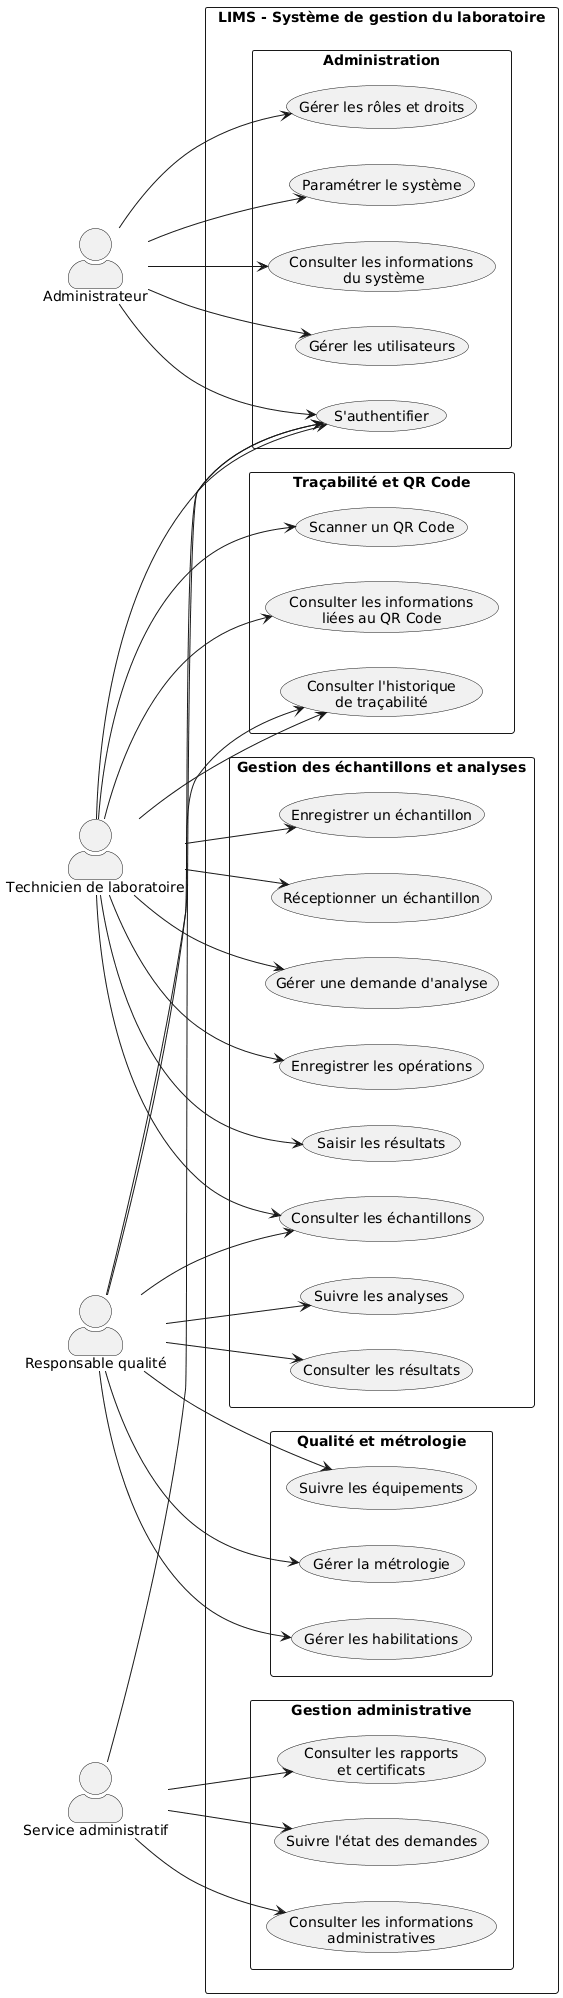
\includegraphics[height=0.78\textheight]{uc-lims.png}
  \caption{Diagramme des cas d'utilisation du LIMS.}
  \label{fig:cas-utilisation}
\end{figure}

\subsection{Diagramme d'activité}

Le diagramme d'activité (figure~\ref{fig:activite-ctaa}) décrit le déroulement global du traitement d'une demande dans le \ac{LIMS}, de l'authentification de l'utilisateur jusqu'à l'archivage des données. Il montre en particulier les deux manières d'identifier un échantillon : par lecture du code \ac{QR}, qui récupère automatiquement les analyses associées, ou par recherche manuelle.

\begin{figure}[H]
  \centering
  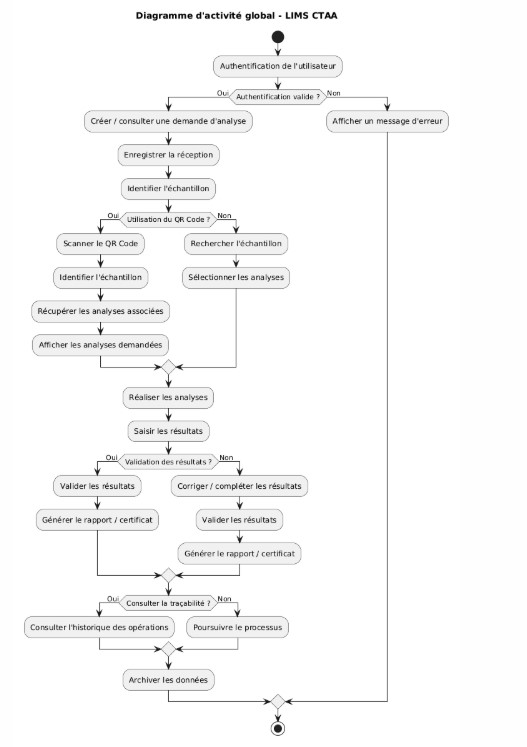
\includegraphics[height=0.72\textheight]{activite-lims.jpg}
  \caption{Diagramme d'activité du traitement d'une demande dans le LIMS.}
  \label{fig:activite-ctaa}
\end{figure}

%-------------------------------------------------------------
\section{Analyse des besoins de Pharmaghreb}
%-------------------------------------------------------------

\subsection{Acteurs}

L'objectif est de récupérer automatiquement les mesures d'un équipement de laboratoire existant, une balance communiquant par liaison série \ac{RS-232}, sans modifier son fonctionnement. Quatre acteurs interagissent avec le module d'acquisition :
\begin{itemize}
    \item \textbf{l'opérateur de laboratoire}, qui s'identifie et réalise les pesées ;
    \item \textbf{l'administrateur technique}, qui installe le module et configure sa connexion réseau ;
    \item \textbf{la balance}, acteur secondaire qui fournit les mesures ;
    \item \textbf{le système d'information} (serveur, application de supervision ou \ac{LIMS}), acteur secondaire qui récupère les données.
\end{itemize}

\subsection{Besoins fonctionnels}
\begin{itemize}
    \item acquérir automatiquement les mesures de la balance, pour supprimer la saisie manuelle ;
    \item identifier l'opérateur par badge \ac{NFC}, afin de rattacher chaque mesure à une personne ;
    \item informer l'opérateur localement de l'état du dispositif (connexion réseau, adresse \ac{IP}, dernière mesure) ;
    \item mettre les mesures à disposition du système d'information via le réseau \ac{Wi-Fi} ;
    \item permettre la configuration du réseau sans reprogrammation, et sa réinitialisation par un bouton.
\end{itemize}

\subsection{Besoins non fonctionnels}
\begin{itemize}
    \item \textbf{Non-intrusivité} : ne modifier ni le matériel ni le paramétrage métrologique de la balance ;
    \item \textbf{Compatibilité électrique} : adapter les niveaux du \ac{RS-232} (jusqu'à $\pm$15~V) aux niveaux logiques 3,3~V du microcontrôleur \citep{tia232} ;
    \item \textbf{Fiabilité des données} : transmettre la valeur exacte affichée par la balance, avec son unité et son état de stabilité ;
    \item \textbf{Faible coût et faible encombrement}, pour pouvoir équiper plusieurs postes ;
    \item \textbf{Évolutivité} : pouvoir connecter d'autres équipements et alimenter à terme un \ac{LIMS}.
\end{itemize}

\subsection{Diagramme des cas d'utilisation}

La figure~\ref{fig:uc-pharmaghreb} présente les cas d'utilisation du module d'acquisition.

\begin{figure}[H]
\centering
\begin{tikzpicture}
  \node[draw=bleu, thick, rounded corners=4pt, minimum width=8.2cm, minimum height=10.6cm,
        label={[font=\small\bfseries, text=bleu]below:Module d'acquisition}] (sys) at (0,0) {};
  \node[cu] (nfc)  at (0, 3.9)  {S'identifier par badge NFC};
  \node[cu] (pes)  at (0, 2.4)  {Effectuer une pesée};
  \node[cu] (acq)  at (0, 0.9)  {Acquérir la mesure};
  \node[cu] (etat) at (0,-0.6)  {Consulter l'état du dispositif};
  \node[cu] (get)  at (0,-2.1)  {Récupérer les mesures};
  \node[cu] (cfg)  at (0,-3.6)  {Configurer le réseau Wi-Fi};

  \bonhomme{(-6.2,2.6)}{Opérateur}
  \bonhomme{(-6.2,-3.0)}{Administrateur\\technique}
  \bonhomme{(6.2,1.5)}{Balance}
  \bonhomme{(6.2,-2.4)}{Système\\d'information}

  \draw[thick, gris] (-5.85,2.8) -- (nfc.west);
  \draw[thick, gris] (-5.85,2.8) -- (pes.west);
  \draw[thick, gris] (-5.85,2.8) -- (etat.west);
  \draw[thick, gris] (-5.85,-2.8) -- (cfg.west);
  \draw[thick, gris] (-5.85,-2.8) -- (etat.west);
  \draw[thick, gris] (5.85,1.7) -- (acq.east);
  \draw[thick, gris] (5.85,-2.2) -- (get.east);
  \draw[fleche, dashed] (pes) -- node[right, etiq] {«include»} (acq);
\end{tikzpicture}
\caption{Diagramme des cas d'utilisation du module d'acquisition (Pharmaghreb).}
\label{fig:uc-pharmaghreb}
\end{figure}

%-------------------------------------------------------------
\section*{Conclusion}
\addcontentsline{toc}{section}{Conclusion}
%-------------------------------------------------------------

Ce chapitre a défini les acteurs et les besoins fonctionnels et non fonctionnels du \ac{LIMS} et de son module de traçabilité, modélisés par des diagrammes de cas d'utilisation et d'activité. Il a ensuite précisé les besoins du module d'acquisition de Pharmaghreb. Le chapitre suivant présente la conception des deux solutions.

\chapter{Conception}
\label{chap:conception}

Ce chapitre présente la conception des deux solutions. Pour le \ac{CTAA}, nous décrivons l'architecture du module de traçabilité, son principe de fonctionnement, la structure des codes et l'algorithme qui les interprète, les échanges entre ses composants et le modèle de données sur lequel il s'appuie. Pour Pharmaghreb, nous détaillons l'architecture matérielle du module d'acquisition, le choix des composants, le câblage, le protocole de communication avec la balance et la logique du programme embarqué.

%=============================================================
\section{Conception du module de traçabilité (CTAA)}
%=============================================================

\subsection{Architecture logicielle}

Le module de traçabilité est intégré au \ac{LIMS}. Il repose sur une architecture en trois niveaux (figure~\ref{fig:architecture-tracabilite}) :
\begin{itemize}
    \item \textbf{le niveau présentation} (\ac{HTML}, CSS et JavaScript) s'exécute dans le navigateur. Il reçoit le contenu lu par la douchette, qui se comporte comme un clavier, et l'envoie au serveur par une requête \ac{AJAX}, c'est-à-dire sans recharger la page ;
    \item \textbf{le niveau application} (\ac{PHP}) reçoit la requête, identifie le type de code, construit et exécute les requêtes \ac{SQL}, puis renvoie le résultat au format \ac{JSON} \citep{php} ;
    \item \textbf{le niveau données} est la base PostgreSQL du \ac{LIMS}, qui contient les demandes, les échantillons, les réceptions, les préparations, les lots et les utilisateurs \citep{postgresql}.
\end{itemize}

\begin{figure}[H]
\centering
\begin{tikzpicture}
  \node[bloc=2.6cm] (douchette) at (0,3.0) {\textbf{Douchette}\\{\scriptsize codes QR et codes-barres}};
  \node[bloc=3.0cm, minimum height=2.8cm] (client) at (0,0)
       {\textbf{Navigateur}\\[3pt] HTML / CSS\\ JavaScript\\ {\scriptsize affichage dynamique}};
  \node[blocvert=3.4cm, minimum height=2.8cm] (srv) at (5.4,0)
       {\textbf{Serveur web}\\[3pt] Back-end PHP\\ {\scriptsize identification du code,\\ requêtes SQL,\\ mise en forme JSON}};
  \node[blocorange=3.0cm, minimum height=2.8cm] (bd) at (10.6,0)
       {\textbf{PostgreSQL}\\[3pt] Base du LIMS\\ {\scriptsize réceptions, préparations,\\ échantillons, lots,\\ utilisateurs}};
  \draw[fleche] (douchette) -- node[right, etiq] {chaîne lue\\(émulation clavier)} (client);
  \draw[fleche] ([yshift=5mm]client.east) -- node[above, etiq] {requête AJAX\\(HTTP)} ([yshift=5mm]srv.west);
  \draw[fleche] ([yshift=-5mm]srv.west) -- node[below, etiq] {réponse\\JSON} ([yshift=-5mm]client.east);
  \draw[fleche] ([yshift=5mm]srv.east) -- node[above, etiq] {requêtes\\SQL} ([yshift=5mm]bd.west);
  \draw[fleche] ([yshift=-5mm]bd.west) -- node[below, etiq] {lignes de\\résultat} ([yshift=-5mm]srv.east);
  \node[etiq, font=\small\bfseries] at (0,-2.0)    {Présentation};
  \node[etiq, font=\small\bfseries] at (5.4,-2.0)  {Application};
  \node[etiq, font=\small\bfseries] at (10.6,-2.0) {Données};
\end{tikzpicture}
\caption{Architecture en trois niveaux du module de traçabilité.}
\label{fig:architecture-tracabilite}
\end{figure}

Cette séparation présente trois avantages : l'interface reste réactive, car seules les données utiles transitent entre le navigateur et le serveur ; la logique d'interprétation des codes est centralisée côté serveur ; enfin, l'ajout d'un nouveau type de code ne modifie que le niveau application.

\subsection{Principe de fonctionnement}

Le module donne un accès immédiat aux informations liées aux opérations du laboratoire. Il propose deux modes de recherche, sélectionnés par l'utilisateur :
\begin{itemize}
    \item \textbf{la recherche par code} : l'utilisateur scanne l'étiquette d'un élément géré par le \ac{LIMS}. Dans le module de gestion des demandes, les étiquettes d'échantillons portent un code \ac{QR}, généré par le bouton « Gén. étiquette » de la demande ; dans les autres modules (réceptions, préparations, stocks), les étiquettes portent pour l'instant un code-barres. La douchette lit indifféremment les deux et transmet leur contenu sous forme de chaîne de caractères ;
    \item \textbf{la recherche par numéro de série} : l'utilisateur saisit ou scanne un numéro de série ou de lot (par exemple celui d'un réactif) afin de retrouver toutes les réceptions qui le concernent.
\end{itemize}

Le traitement se déroule ensuite en quatre étapes : \textbf{lecture} du code, \textbf{identification} de son type, \textbf{interrogation} de la base de données et \textbf{affichage} du résultat ou d'un message d'erreur. Les sections suivantes détaillent ces étapes.

\subsection{Structure des codes et règles d'identification}

Le contenu d'un code est organisé autour du séparateur «~\texttt{\#}~». Le serveur découpe la chaîne en éléments et déduit le type de code d'après leur nombre et certaines valeurs (tableau~\ref{tab:structure-qr}).

\begin{table}[H]
\centering
\renewcommand{\arraystretch}{1.3}
\begin{tabularx}{\textwidth}{|p{6.8cm}|Y|}
\hline
\enteteligne \entete{Contenu du code} & \entete{Interprétation} \\ \hline
Sept éléments, le troisième vaut «~\texttt{CTA}~» & Code de préparation \\ \hline
Sept éléments, le troisième est différent de «~\texttt{CTA}~» & Code de réception \\ \hline
Deux éléments & Analyse complémentaire (présence d'une date) pour déterminer le processus associé \\ \hline
Autre structure & Code incorrect : message d'erreur \\ \hline
\end{tabularx}
\caption{Règles d'identification des codes par le module de traçabilité.}
\label{tab:structure-qr}
\end{table}

Le tableau~\ref{tab:exemple-code} décompose, à titre d'exemple, le code de préparation \texttt{test\#dev\#CTA\#260808\#100\#2026-08-08\#2206214830101} utilisé lors des tests.

% À VÉRIFIER : signification exacte des éléments 1, 2 et 5.
\begin{table}[H]
\centering
\renewcommand{\arraystretch}{1.25}
\begin{tabular}{|c|l|l|}
\hline
\enteteligne \entete{Position} & \entete{Valeur} & \entete{Signification} \\ \hline
1--2 & \texttt{test}, \texttt{dev} & Désignation du produit préparé \\ \hline
3 & \texttt{CTA} & Marqueur d'un code de préparation \\ \hline
4 & \texttt{260808} & Numéro de lot \\ \hline
5 & \texttt{100} & Quantité conditionnée \\ \hline
6 & \texttt{2026-08-08} & Date de préparation \\ \hline
7 & \texttt{2206214830101} & Numéro d'étiquette \\ \hline
\end{tabular}
\caption{Exemple de décomposition d'un code de préparation.}
\label{tab:exemple-code}
\end{table}

La figure~\ref{fig:algo-identification} présente l'algorithme d'identification exécuté par le serveur.

\begin{figure}[H]
\centering
\begin{tikzpicture}[
    decision/.append style={text width=2.2cm, font=\scriptsize},
    bloc/.append style={font=\scriptsize}]
  \node[debutfin] (start) at (0,0) {Code reçu};
  \node[decision] (mode) at (0,-1.7) {Mode de recherche ?};
  \node[bloc=2.8cm] (serie) at (-4.6,-1.7) {Rechercher les réceptions du lot};
  \node[bloc=2.8cm] (split) at (0,-3.4) {Découper la chaîne selon «~\#~»};
  \node[decision] (n7) at (0,-5.1) {Sept éléments ?};
  \node[decision] (cta) at (-4.6,-5.1) {3\textsuperscript{e} élément = CTA ?};
  \node[bloc=2.2cm] (prep) at (-6.4,-7.0) {Préparation};
  \node[bloc=2.2cm] (recep) at (-2.8,-7.0) {Réception};
  \node[decision] (n2) at (0,-7.0) {Deux éléments ?};
  \node[bloc=2.8cm] (date) at (4.6,-7.0) {Analyse complémentaire (date)};
  \node[blocorange=2.8cm] (err) at (0,-9.0) {Code incorrect :\\message d'erreur};
  \node[bloc=3.2cm] (sql) at (-4.6,-9.0) {Requête SQL selon le type};
  \node[decision] (vide) at (-4.6,-10.9) {Résultat vide ?};
  \node[blocvert=2.8cm] (aff) at (0,-10.9) {Afficher le tableau de traçabilité};

  \draw[fleche] (start) -- (mode);
  \draw[fleche] (mode) -- node[above, etiq] {numéro\\de série} (serie);
  \draw[fleche] (mode) -- node[right, etiq] {code} (split);
  \draw[fleche] (split) -- (n7);
  \draw[fleche] (n7) -- node[above, etiq] {oui} (cta);
  \draw[fleche] (n7) -- node[right, etiq] {non} (n2);
  \draw[fleche] (cta) -| node[pos=0.2, above, etiq] {oui} (prep);
  \draw[fleche] (cta) -| node[pos=0.2, above, etiq] {non} (recep);
  \draw[fleche] (n2) -- node[above, etiq] {oui} (date);
  \draw[fleche] (n2) -- node[right, etiq] {non} (err);
  \draw[fleche] (prep) |- (sql);
  \draw[fleche] (recep) |- (sql);
  \draw[fleche] (date.south) |- ++(0,-0.6) -| ([xshift=6mm]sql.north);
  \draw[fleche] (serie.west) -- ++(-2.4,0) |- (sql.west);
  \draw[fleche] (sql) -- (vide);
  \draw[fleche] (vide) -- node[above, etiq] {non} (aff);
  \draw[fleche] (vide.south) -- ++(0,-0.4) -| node[pos=0.25, below, etiq] {oui} ([xshift=8mm]err.south);
\end{tikzpicture}
\caption{Algorithme d'identification et de traitement d'un code.}
\label{fig:algo-identification}
\end{figure}

\subsection{Diagramme de séquence}

Le diagramme de séquence de la figure~\ref{fig:sequence-scan} décrit les échanges entre les composants lors de la lecture d'un code, dans le cas nominal et dans le cas d'un code incorrect.

\begin{figure}[H]
\centering
\resizebox{\textwidth}{!}{%
\begin{tikzpicture}[
    tete/.style={draw=bleu, fill=bleuclair, font=\small\bfseries, minimum height=8mm, minimum width=2.3cm, align=center},
    msg/.style={-{Stealth[length=2.2mm]}, thick, draw=gris},
    ret/.style={-{Stealth[length=2.2mm]}, thick, dashed, draw=gris},
    lab/.style={font=\scriptsize, above, align=center}]
  \foreach \x/\n/\t in {0/T/Technicien, 3/D/Douchette, 6.2/I/Interface web, 9.6/S/Serveur PHP, 13/B/PostgreSQL} {
    \node[tete] (\n) at (\x,0) {\t};
    \draw[dashed, gris!70] (\n.south) -- (\x,-10.6);
  }
  \draw[msg] (0,-1.1) -- node[lab] {scanner l'étiquette} (3,-1.1);
  \draw[msg] (3,-1.9) -- node[lab] {chaîne lue + Entrée} (6.2,-1.9);
  \draw[msg] (6.2,-2.7) -- node[lab] {requête AJAX (code, mode)} (9.6,-2.7);
  \draw[msg] (9.6,-3.3) -- ++(0.8,0) -- ++(0,-0.5) -- node[font=\scriptsize, right, align=left, pos=0] {\hspace{8mm}découper la chaîne,\\\hspace{8mm}identifier le type} ++(-0.8,0);
  % Fragment alt
  \draw[draw=orange, thick] (-1.3,-4.4) rectangle (14.3,-10.2);
  \node[draw=orange, fill=orange!10, font=\scriptsize\bfseries, anchor=north west] at (-1.3,-4.4) {alt};
  \node[font=\scriptsize\itshape, anchor=west] at (-0.6,-4.75) {[type reconnu]};
  \draw[msg] (9.6,-5.2) -- node[lab] {requête SQL (identifiant)} (13,-5.2);
  \draw[ret] (13,-6.0) -- node[lab] {lignes de traçabilité} (9.6,-6.0);
  \draw[ret] (9.6,-6.8) -- node[lab] {réponse JSON (données)} (6.2,-6.8);
  \draw[ret] (6.2,-7.6) -- node[lab] {tableau de traçabilité} (0,-7.6);
  \draw[draw=orange, dashed] (-1.3,-8.2) -- (14.3,-8.2);
  \node[font=\scriptsize\itshape, anchor=west] at (-0.6,-8.5) {[code incorrect ou inconnu]};
  \draw[ret] (9.6,-9.1) -- node[lab] {réponse JSON (erreur)} (6.2,-9.1);
  \draw[ret] (6.2,-9.8) -- node[lab] {message « code incorrect »} (0,-9.8);
\end{tikzpicture}}
\caption{Diagramme de séquence de la lecture d'un code.}
\label{fig:sequence-scan}
\end{figure}

\subsection{Modèle de données}

La figure~\ref{fig:modele-donnees} présente le modèle conceptuel des données manipulées par le module. Une \emph{demande} concerne un ou plusieurs \emph{échantillons}, chacun faisant l'objet d'une ou plusieurs \emph{analyses}. Une \emph{réception} regroupe des lignes d'articles (réactifs, consommables), chacune rattachée à un \emph{lot} ; une \emph{préparation} utilise un ou plusieurs lots. Enfin, chaque \emph{opération} est réalisée par un \emph{utilisateur} et porte sur un échantillon ou une préparation : c'est l'ensemble de ces opérations qui constitue l'historique de traçabilité.

\begin{figure}[H]
\centering
\begin{tikzpicture}[
    classe/.style={rectangle split, rectangle split parts=2, draw=bleu, thick,
                   rectangle split part fill={bleuclair,white}, font=\scriptsize,
                   text width=3.2cm, align=left, inner sep=3pt},
    assoc/.style={thick, draw=gris},
    mult/.style={font=\scriptsize, text=gris}]
  \node[classe] (dem) at (0,0)    {\centering\textbf{Demande}\nodepart{second}numéro\\date\\demandeur\\statut};
  \node[classe] (ech) at (5.4,0)  {\centering\textbf{Échantillon}\nodepart{second}identifiant\\désignation du produit\\date de réception\\code QR};
  \node[classe] (ana) at (10.8,0) {\centering\textbf{Analyse}\nodepart{second}code\\désignation\\méthode\\résultat, statut};
  \node[classe] (usr) at (0,-4.2)    {\centering\textbf{Utilisateur}\nodepart{second}identifiant\\nom\\rôle};
  \node[classe] (ope) at (5.4,-4.2)  {\centering\textbf{Opération}\nodepart{second}type\\date et heure\\commentaire};
  \node[classe] (pre) at (10.8,-4.2) {\centering\textbf{Préparation}\nodepart{second}produit\\numéro d'étiquette\\date\\magasin};
  \node[classe] (rec) at (0,-8.4)    {\centering\textbf{Réception}\nodepart{second}numéro\\date\\fournisseur};
  \node[classe] (lig) at (5.4,-8.4)  {\centering\textbf{Ligne de réception}\nodepart{second}article\\quantité demandée\\quantité reçue\\date limite (DLC)};
  \node[classe] (lot) at (10.8,-8.4) {\centering\textbf{Lot}\nodepart{second}numéro de lot / série\\fournisseur};

  \draw[assoc] (dem) -- node[above, etiq] {concerne} node[mult, pos=0.12, below] {1} node[mult, pos=0.85, below] {1..*} (ech);
  \draw[assoc] (ech) -- node[above, etiq] {fait l'objet de} node[mult, pos=0.12, below] {*} node[mult, pos=0.85, below] {1..*} (ana);
  \draw[assoc] (usr) -- node[above, etiq] {réalise} node[mult, pos=0.12, below] {1} node[mult, pos=0.85, below] {*} (ope);
  \draw[assoc] (ope) -- node[left, etiq] {porte sur} node[mult, pos=0.15, right] {*} node[mult, pos=0.85, right] {0..1} (ech);
  \draw[assoc] (ope) -- node[above, etiq] {porte sur} node[mult, pos=0.12, below] {*} node[mult, pos=0.85, below] {0..1} (pre);
  \draw[assoc] (usr) -- node[left, etiq] {enregistre} node[mult, pos=0.15, right] {1} node[mult, pos=0.85, right] {*} (rec);
  \draw[assoc] (rec) -- node[above, etiq] {contient} node[mult, pos=0.12, below] {1} node[mult, pos=0.85, below] {1..*} (lig);
  \draw[assoc] (lig) -- node[above, etiq] {référence} node[mult, pos=0.12, below] {*} node[mult, pos=0.85, below] {1} (lot);
  \draw[assoc] (pre) -- node[left, etiq] {utilise} node[mult, pos=0.15, right] {*} node[mult, pos=0.85, right] {1..*} (lot);
\end{tikzpicture}
\caption{Modèle conceptuel des données du module de traçabilité.}
\label{fig:modele-donnees}
\end{figure}

\subsection{Accès aux données}

Dans le \ac{LIMS}, chaque objet métier (demande, réception, lot, préparation, etc.) est stocké comme un \emph{document} appartenant à une \emph{famille}, et chaque famille correspond à une table de la base (\texttt{doc952028} pour les lots, \texttt{doc13162797} pour les réceptions, etc.). Deux choix de conception en découlent :
\begin{itemize}
    \item \textbf{résolution dynamique des familles} : le module ne code pas en dur les numéros de tables ; il retrouve l'identifiant de chaque famille à partir de son nom (\texttt{lot\_matiere}, \texttt{prd}, \texttt{emballage}, \texttt{tracabilite\_produit}, etc.). Il reste ainsi valable d'une instance du \ac{LIMS} à l'autre, et les paramètres de connexion sont lus dans un fichier de configuration (\texttt{config.ini}) ;
    \item \textbf{dépliage des champs multivalués} : une réception stocke ses lignes (articles, quantités demandées et reçues, \ac{DLC}) sous forme de listes séparées par des retours à la ligne. La requête les déplie en lignes distinctes grâce à la fonction PostgreSQL \texttt{regexp\_split\_to\_table}.
\end{itemize}

Le listing~\ref{lst:requete-serie} présente la requête de la recherche par numéro de série. Elle retrouve d'abord les réceptions associées au lot recherché, en excluant les documents supprimés (\texttt{doctype = 'Z'}), puis déplie leurs lignes.

\begin{lstlisting}[language=SQL, caption={Requête de traçabilité par numéro de série (lot \texttt{CS07251350}).}, label={lst:requete-serie}]
WITH data AS (
    SELECT t_doc_app_recep AS id_recep
    FROM doc952028 AS lot              -- famille des lots
    WHERE lot.doctype != 'Z'           -- exclut les documents supprimés
      AND lot.t_lot = 'CS07251350'     -- numéro de série recherché
)
SELECT recep.id AS id_recep,
       recep.t_user,
       regexp_split_to_table(recep.t_product, E'\n')       AS t_product,
       regexp_split_to_table(recep.qte_dem::text, E'\n')   AS qte_dem,
       regexp_split_to_table(recep.qte_recu::text, E'\n')  AS qte_recu,
       regexp_split_to_table(recep.date_dlc::text, E'\n')  AS date_dlc
FROM data
JOIN doc13162797 AS recep              -- famille des réceptions
  ON recep.id::text = data.id_recep::text;
\end{lstlisting}

%=============================================================
\section{Conception du module d'acquisition (Pharmaghreb)}
%=============================================================

\subsection{Architecture matérielle}

Le module d'acquisition relie directement le monde physique au système d'information, dans une logique d'Internet industriel des objets (\ac{IIoT}). Il joue le rôle de nœud \emph{edge} : il reçoit les trames de la balance, en extrait la mesure, l'associe à l'opérateur et la met à disposition sur le réseau (figure~\ref{fig:archi-materielle}).

\begin{figure}[H]
\centering
\begin{tikzpicture}
  \node[blocorange=2.2cm, minimum height=1.6cm] (bal) at (0,0) {\textbf{Balance}\\Mettler Toledo\\XSR205};
  \node[bloc=2.2cm, minimum height=1.6cm] (max) at (3.8,0) {\textbf{MAX3232}\\{\scriptsize convertisseur\\RS-232 / TTL}};
  \node[blocvert=2.6cm, minimum height=2.4cm] (mcu) at (7.6,0) {\textbf{NodeMCU}\\ESP-12E\\(ESP8266)\\{\scriptsize UART, I$^2$C, Wi-Fi}};
  \node[bloc=2.4cm] (nfc) at (7.6,3.1) {\textbf{PN532}\\{\scriptsize lecteur NFC}};
  \node[bloc=2.0cm] (btn) at (7.6,-3.0) {\textbf{Bouton}\\{\scriptsize réinitialisation}};
  \node[bloc=2.4cm] (bss) at (11.8,1.4) {\textbf{BSS138}\\{\scriptsize adaptateur\\3,3 V / 5 V}};
  \node[bloc=2.4cm] (lcd) at (11.8,3.6) {\textbf{LCD 16$\times$2}\\{\scriptsize affichage local}};
  \node[blocorange=2.4cm, minimum height=1.3cm] (si) at (11.8,-1.6) {\textbf{Système\\d'information}\\{\scriptsize serveur, LIMS}};

  \draw[doublefleche] (bal) -- node[above, etiq] {RS-232\\(DB9)} node[below, etiq] {$\pm$12 V} (max);
  \draw[doublefleche] (max) -- node[above, etiq] {UART} node[below, etiq] {3,3 V} (mcu);
  \draw[doublefleche] (nfc) -- node[right, etiq] {I$^2$C (adresse 0x24)\\IRQ, RSTO} (mcu);
  \draw[fleche] (btn) -- node[right, etiq] {GPIO} (mcu);
  \draw[doublefleche] (mcu.north east) |- node[pos=0.75, above, etiq] {I$^2$C 3,3 V} (bss.west);
  \draw[doublefleche] (bss) -- node[right, etiq] {I$^2$C 5 V} (lcd);
  \draw[fleche] (mcu.south east) |- node[pos=0.75, above, etiq] {Wi-Fi, HTTP} node[pos=0.75, below, etiq] {\texttt{/getData} (JSON)} (si.west);
\end{tikzpicture}
\caption{Architecture matérielle du module d'acquisition.}
\label{fig:archi-materielle}
\end{figure}

\subsection{Choix des composants}

Le tableau~\ref{tab:composants} justifie le choix de chaque composant.

\begin{table}[H]
\centering
\renewcommand{\arraystretch}{1.25}
\begin{tabularx}{\textwidth}{|p{3.3cm}|Y|Y|}
\hline
\enteteligne \entete{Composant} & \entete{Fonction} & \entete{Justification du choix} \\ \hline
NodeMCU ESP-12E (ESP8266) & Unité de traitement : réception des trames, logique applicative, serveur HTTP & Wi-Fi intégré, faible coût, programmation simple, interfaces UART et I$^2$C disponibles \citep{esp8266} \\ \hline
MAX3232 & Conversion des niveaux RS-232 ($\pm$12 V) en niveaux TTL 3,3 V & Fonctionne en 3,3 V, compatible avec l'ESP8266 ; protège le microcontrôleur \citep{max3232} \\ \hline
PN532 & Lecture des badges NFC des opérateurs & Mode I$^2$C, alimentation 3,3 V, compatible avec les badges MIFARE et NTAG \citep{pn532} \\ \hline
LCD 16$\times$2 (I$^2$C) & Affichage de l'état du réseau, de l'adresse IP et de la dernière mesure & IHM simple et lisible ; seulement deux fils grâce au bus I$^2$C \\ \hline
BSS138 & Adaptation des niveaux logiques entre le bus I$^2$C 3,3 V et l'écran 5 V & Adaptateur bidirectionnel adapté aux lignes SDA et SCL \\ \hline
Bouton poussoir & Effacement de la configuration Wi-Fi (appui de 5 s) & Permet de reconfigurer le module sans le reprogrammer \\ \hline
\end{tabularx}
\caption{Composants du module d'acquisition et justification de leur choix.}
\label{tab:composants}
\end{table}

\subsection{Schéma de câblage}

La figure~\ref{fig:cablage} présente le schéma de câblage du prototype et le tableau~\ref{tab:cablage} détaille les connexions. Le PN532 et l'écran \ac{LCD} partagent le même bus \ac{I2C} (broches D1 et D2) ; l'écran, alimenté en 5~V, y est raccordé à travers l'adaptateur BSS138.

\begin{figure}[H]
  \centering
  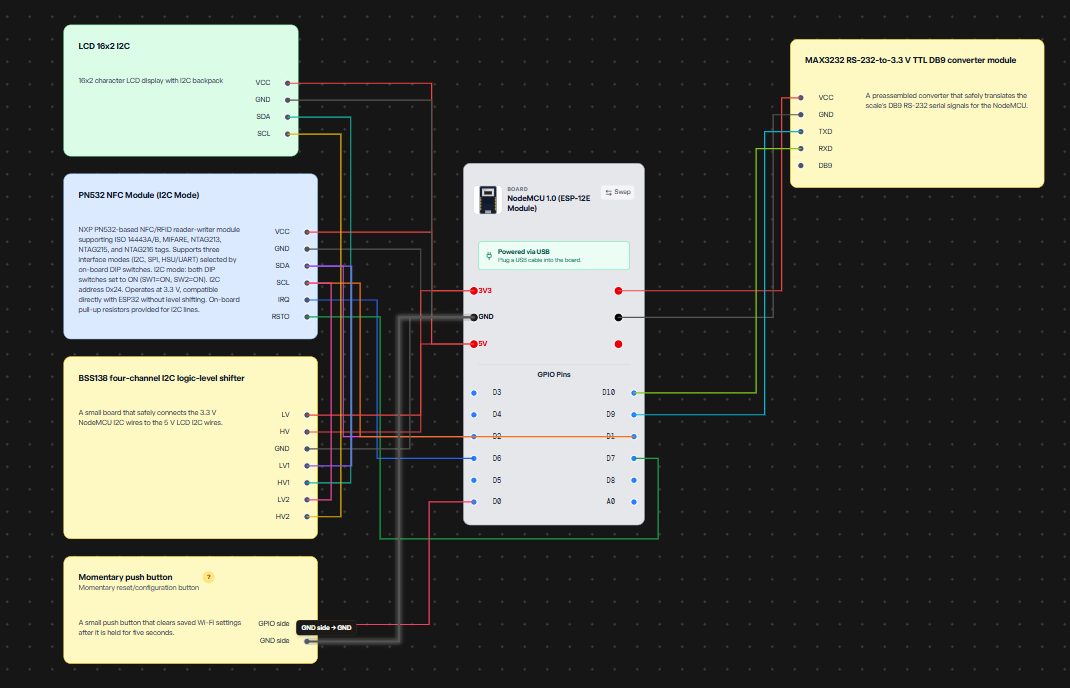
\includegraphics[width=\textwidth]{cablage-prototype.png}
  \caption{Schéma de câblage du module d'acquisition.}
  \label{fig:cablage}
\end{figure}

\begin{table}[H]
\centering
\renewcommand{\arraystretch}{1.2}
\begin{tabular}{|l|l|l|l|}
\hline
\enteteligne \entete{Composant} & \entete{Broche} & \entete{NodeMCU} & \entete{Rôle} \\ \hline
\multirow{4}{*}{MAX3232} & VCC / GND & 3V3 / GND & Alimentation \\
 & TXD & D9 (GPIO3, RX) & Réception des trames de la balance \\
 & RXD & D10 (GPIO1, TX) & Envoi des commandes à la balance \\
 & DB9 & -- & Liaison RS-232 avec la balance \\ \hline
\multirow{4}{*}{PN532} & VCC / GND & 3V3 / GND & Alimentation \\
 & SDA / SCL & D2 / D1 & Bus I$^2$C \\
 & IRQ & D6 & Signal de détection d'un badge \\
 & RSTO & D7 & Réinitialisation du lecteur \\ \hline
\multirow{2}{*}{BSS138} & LV / HV & 3V3 / 5V & Références de tension \\
 & LV1, LV2 / HV1, HV2 & D2, D1 / LCD & Adaptation de SDA et SCL \\ \hline
LCD 16$\times$2 & VCC / GND & 5V / GND & Alimentation \\ \hline
Bouton & GPIO / GND & D0 / GND & Effacement de la configuration Wi-Fi \\ \hline
\end{tabular}
\caption{Connexions du module d'acquisition.}
\label{tab:cablage}
\end{table}

La liaison série croise les signaux : la sortie TXD du MAX3232 est reliée à l'entrée RX du NodeMCU, et son entrée RXD à la sortie TX. Cette liaison utilise l'UART matériel de l'ESP8266, également relié au port USB de programmation : en fonctionnement, il est réservé à la balance, et le programme est téléversé balance débranchée.

\subsection{Protocole de communication avec la balance}

\subsubsection*{Paramètres de la liaison série}

Une liaison \ac{RS-232} ne fonctionne que si les deux extrémités utilisent les mêmes paramètres : débit, nombre de bits de données, parité et bits d'arrêt \citep{tia232}. Le module est configuré selon le paramétrage de l'interface de la balance.
% À VÉRIFIER : remplacer par les paramètres réellement configurés sur la balance.
Nous avons retenu une configuration 9600~bauds, 8~bits de données, sans parité, 1~bit d'arrêt (8N1).

\subsubsection*{Jeu de commandes MT-SICS}

Les balances Mettler Toledo communiquent selon le protocole \ac{MT-SICS} \citep{mtsics}. Le module envoie une commande textuelle terminée par un retour chariot et un saut de ligne, et la balance répond par une trame de même format. Le tableau~\ref{tab:mtsics} présente les commandes utilisées.

\begin{table}[H]
\centering
\renewcommand{\arraystretch}{1.25}
\begin{tabularx}{\textwidth}{|c|Y|l|}
\hline
\enteteligne \entete{Commande} & \entete{Effet} & \entete{Exemple de réponse} \\ \hline
\texttt{S} & Envoie la prochaine valeur de poids \emph{stable} & \texttt{S S \ \ \ \ 100.00 g} \\ \hline
\texttt{SI} & Envoie immédiatement la valeur courante, stable ou non & \texttt{S D \ \ \ \ \ 99.87 g} \\ \hline
\texttt{Z} & Remet la balance à zéro & \texttt{Z A} \\ \hline
\end{tabularx}
\caption{Commandes MT-SICS utilisées par le module.}
\label{tab:mtsics}
\end{table}

Le deuxième champ de la réponse indique l'état de la mesure : \texttt{S} pour une valeur stable, \texttt{D} pour une valeur dynamique (instable), \texttt{I} si la commande ne peut pas être exécutée, \texttt{+} ou \texttt{-} en cas de dépassement de la plage de pesée. Le module n'enregistre comme mesure que les valeurs stables, ce qui garantit que la donnée transmise correspond à une pesée valide.

\subsubsection*{Données mises à disposition}

Le module expose un point d'accès \ac{HTTP}, \texttt{/getData}, que le système d'information interroge pour récupérer la dernière mesure au format \ac{JSON}. Le tableau~\ref{tab:donnees-json} décrit les données transmises.

% À ADAPTER : aligner les noms de champs sur ceux du programme embarqué.
\begin{table}[H]
\centering
\renewcommand{\arraystretch}{1.2}
\begin{tabularx}{\textwidth}{|l|Y|l|}
\hline
\enteteligne \entete{Donnée} & \entete{Description} & \entete{Exemple} \\ \hline
Valeur & Valeur numérique de la pesée & \texttt{100.00} \\ \hline
Unité & Unité renvoyée par la balance & \texttt{g} \\ \hline
Stabilité & État de la mesure (stable ou non) & \texttt{S} \\ \hline
Opérateur & Identifiant du dernier badge NFC lu & \texttt{04A1B2C3} \\ \hline
Horodatage & Instant d'acquisition de la mesure & \texttt{2026-09-23 14:27:20} \\ \hline
\end{tabularx}
\caption{Données transmises par le point d'accès \texttt{/getData}.}
\label{tab:donnees-json}
\end{table}

\subsection{Logique du programme embarqué}

La figure~\ref{fig:organigramme} présente l'organigramme du programme embarqué. Au démarrage, le module initialise ses périphériques et vérifie si le bouton est maintenu pendant cinq secondes, auquel cas il efface la configuration \ac{Wi-Fi}. S'il ne connaît aucun réseau, il ouvre un point d'accès de configuration, qui permet de saisir les identifiants du réseau depuis un téléphone sans reprogrammer le module. Une fois connecté, il affiche son adresse \ac{IP} sur l'écran, puis entre dans sa boucle principale : il mémorise le badge de l'opérateur, traite les trames de la balance et répond aux requêtes du système d'information.

Le module lit l'identifiant du badge et l'associe aux mesures. Le contrôle d'accès par liste de badges autorisés est prévu dans la conception et pourra être activé selon les besoins de Pharmaghreb.

\begin{figure}[H]
\centering
\begin{tikzpicture}[
    decision/.append style={text width=2.0cm, font=\scriptsize},
    bloc/.append style={font=\scriptsize}]
  % Initialisation
  \node[debutfin] (start) at (0,0) {Démarrage};
  \node[bloc=2.8cm] (init) at (0,-1.3) {Initialiser le LCD, le lecteur NFC et l'UART};
  \node[decision] (d1) at (0,-3.0) {Bouton maintenu 5 s ?};
  \node[bloc=2.6cm] (eff) at (3.7,-3.0) {Effacer la configuration Wi-Fi};
  \node[decision] (d2) at (0,-5.2) {Réseau Wi-Fi configuré ?};
  \node[bloc=2.6cm] (ap) at (3.7,-5.2) {Ouvrir le point d'accès de configuration};
  \node[bloc=2.8cm] (cnx) at (0,-7.0) {Se connecter au réseau local};
  \node[bloc=2.8cm] (aff) at (0,-8.3) {Afficher l'état et l'adresse IP};
  % Boucle principale
  \node[decision] (d3) at (9,0) {Badge NFC présenté ?};
  \node[bloc=3.2cm] (a3) at (9,-1.55) {Mémoriser l'identifiant de l'opérateur};
  \node[decision] (d4) at (9,-3.3) {Trame série reçue ?};
  \node[bloc=3.4cm] (a4) at (9,-4.95) {Analyser la trame ; si stable, mémoriser la mesure horodatée et l'afficher};
  \node[decision] (d5) at (9,-6.75) {Requête \texttt{/getData} ?};
  \node[bloc=3.2cm] (a5) at (9,-8.3) {Répondre en JSON};
  \node[font=\scriptsize\bfseries, text=bleu] at (9,1.45) {Boucle principale};

  \draw[fleche] (start) -- (init);
  \draw[fleche] (init) -- (d1);
  \draw[fleche] (d1) -- node[above, etiq] {oui} (eff);
  \draw[fleche] (d1) -- node[right, etiq] {non} (d2);
  \draw[fleche] (eff.south) |- (0,-4.15);
  \draw[fleche] (d2) -- node[above, etiq] {non} (ap);
  \draw[fleche] (d2) -- node[right, etiq] {oui} (cnx);
  \draw[fleche] (ap) |- (cnx);
  \draw[fleche] (cnx) -- (aff);
  \draw[fleche] (aff.east) -- (6.3,-8.3) |- (9,1.0) -- (d3);

  \draw[fleche] (d3) -- node[right, etiq] {oui} (a3);
  \draw[fleche] (a3) -- (d4);
  \draw[fleche] (d3.west) -- node[above, etiq] {non} (7.1,0) |- (9,-2.45);
  \draw[fleche] (d4) -- node[right, etiq] {oui} (a4);
  \draw[fleche] (a4) -- (d5);
  \draw[fleche] (d4.west) -- node[above, etiq] {non} (7.1,-3.3) |- (9,-5.85);
  \draw[fleche] (d5) -- node[right, etiq] {oui} (a5);
  \draw[fleche] (d5.east) -- node[above, etiq] {non} (11.6,-6.75) |- (9,1.0);
  \draw[fleche] (a5.east) -| (11.6,-6.75);
\end{tikzpicture}
\caption{Organigramme du programme embarqué du module d'acquisition.}
\label{fig:organigramme}
\end{figure}

%-------------------------------------------------------------
\section*{Conclusion}
\addcontentsline{toc}{section}{Conclusion}
%-------------------------------------------------------------

Ce chapitre a présenté la conception des deux solutions. Le module de traçabilité repose sur une architecture en trois niveaux, un algorithme d'identification des codes fondé sur leur structure et un modèle de données qui relie demandes, échantillons, réceptions, lots, préparations et opérations. Le module d'acquisition repose sur un microcontrôleur ESP8266 qui dialogue avec la balance selon le protocole \ac{MT-SICS}, identifie l'opérateur par badge \ac{NFC} et met les mesures à disposition par \ac{Wi-Fi}. Le chapitre suivant présente la réalisation de ces deux solutions.

\chapter{Réalisation}
\label{chap:realisation}

Ce chapitre présente la réalisation des deux solutions. Après une description de l'environnement de travail, nous présentons le déploiement et le paramétrage du \ac{LIMS} au \ac{CTAA}, les interfaces du module de traçabilité, les tests de validation et la formation des utilisateurs. Nous exposons ensuite l'étude des équipements de Pharmaghreb, la réalisation du module d'acquisition et ses tests.

%-------------------------------------------------------------
\section{Environnement de travail}
%-------------------------------------------------------------

Le choix des outils a été guidé par la compatibilité avec l'existant (le \ac{LIMS} de BQube ITs repose sur \ac{PHP} et PostgreSQL), la fiabilité et l'adéquation aux besoins de chaque solution. Le tableau~\ref{tab:environnement} résume les technologies et les outils utilisés.

% À VÉRIFIER : outils de développement embarqué réellement utilisés.
\begin{table}[H]
\centering
\renewcommand{\arraystretch}{1.25}
\begin{tabularx}{\textwidth}{|p{3.6cm}|Y|}
\hline
\enteteligne \entete{Technologie / outil} & \entete{Rôle dans le projet} \\ \hline
\multicolumn{2}{|l|}{\cellcolor{bleuclair}\textbf{Module de traçabilité (CTAA)}} \\ \hline
HTML et CSS & Structure et mise en forme de l'interface : zone de saisie, choix du mode de recherche, tableaux de résultats \\ \hline
JavaScript et AJAX & Récupération de la chaîne lue par la douchette, envoi asynchrone au serveur et affichage dynamique des résultats \\ \hline
PHP & Back-end : identification du type de code, construction des requêtes SQL et mise en forme des réponses JSON \\ \hline
JSON & Format d'échange des données entre le serveur et le navigateur \\ \hline
PostgreSQL 9.6 et SQL & Stockage des données du LIMS et requêtes de traçabilité \\ \hline
phpPgAdmin & Administration de la base, mise au point et vérification des requêtes \\ \hline
Douchette et imprimante d'étiquettes & Lecture des codes QR et codes-barres ; impression des étiquettes \\ \hline
\multicolumn{2}{|l|}{\cellcolor{bleuclair}\textbf{Module d'acquisition (Pharmaghreb)}} \\ \hline
NodeMCU ESP-12E & Carte de développement à base d'ESP8266 \\ \hline
IDE Arduino (cœur ESP8266) & Écriture, compilation et téléversement du programme embarqué \\ \hline
Bibliothèques Wi-Fi, I$^2$C, PN532 et LCD & Connexion réseau, point d'accès de configuration, serveur HTTP, pilotage des périphériques \\ \hline
Outil de schéma électronique & Conception du schéma de câblage (figure~\ref{fig:cablage}) \\ \hline
\end{tabularx}
\caption{Technologies et outils utilisés.}
\label{tab:environnement}
\end{table}

%-------------------------------------------------------------
\section{Déploiement et paramétrage du LIMS au CTAA}
%-------------------------------------------------------------

\subsection{Fonctionnalités mises en place}

Cette première version du \ac{LIMS} couvre les fonctionnalités suivantes :
\begin{itemize}
    \item \textbf{demandes d'analyses} : création et suivi des demandes, enregistrement des analyses demandées, fiches de réception ;
    \item \textbf{échantillons} : identification, enregistrement et suivi tout au long de leur cycle de vie ;
    \item \textbf{produits et analyses} : catalogue des produits, des catégories et des analyses associées ;
    \item \textbf{équipements et métrologie} : suivi des équipements, de leurs contrôles et de leurs étalonnages ;
    \item \textbf{habilitations} : suivi des compétences et des habilitations du personnel ;
    \item \textbf{traçabilité} : module développé dans le cadre de ce projet (section~\ref{sec:module-tracabilite}).
\end{itemize}

\subsection{Création des utilisateurs et des droits d'accès}

Nous avons créé les comptes utilisateurs et attribué à chacun un profil (administrateur, technicien, responsable qualité, service administratif) qui détermine ses droits d'accès. Chaque action enregistrée est ainsi rattachée à son auteur, ce qui renforce la sécurité et la traçabilité.

\subsection{Configuration des produits et des analyses}

Les produits ont été créés et classés par catégories et sous-catégories (préparations alimentaires, sirops, nectars de jus, etc.), puis les analyses correspondantes ont été regroupées en \emph{packs} et associées aux produits. La figure~\ref{fig:configuration} montre par exemple le pack « Identification des colorants synthétiques », qui regroupe dix-sept analyses. Le \ac{LIMS} relie ainsi automatiquement chaque échantillon aux analyses à réaliser.

\begin{figure}[H]
  \centering
  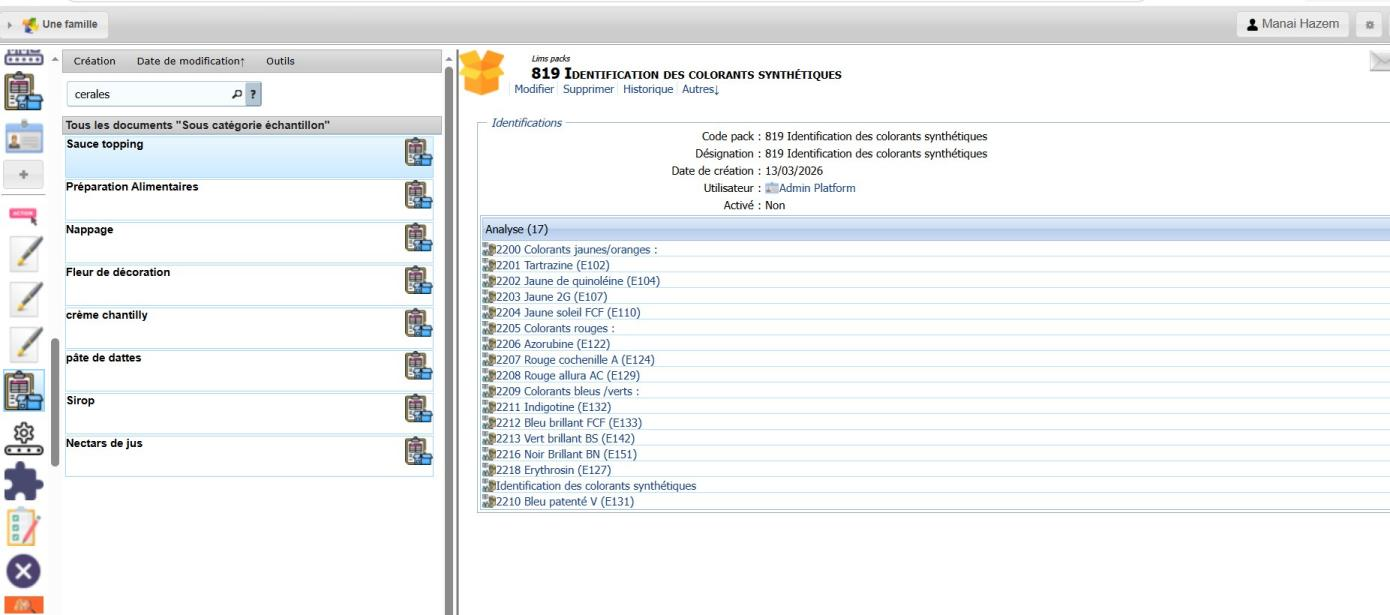
\includegraphics[width=\textwidth]{lims-configuration.png}
  \caption{Configuration des sous-catégories d'échantillons et d'un pack d'analyses.}
  \label{fig:configuration}
\end{figure}

\subsection{Gestion des demandes et étiquetage par code QR}

Le module de gestion des demandes (figure~\ref{fig:demandes}) permet d'enregistrer une demande client, d'y associer les échantillons et les analyses, de générer la fiche de réception et d'imprimer les étiquettes. Nous avons configuré l'imprimante et le format des étiquettes afin que chaque échantillon porte un identifiant unique et un code \ac{QR} (figure~\ref{fig:qr-echantillon}). Une fois apposée, l'étiquette relie directement l'échantillon physique à ses informations dans le \ac{LIMS}.

\begin{figure}[H]
  \centering
  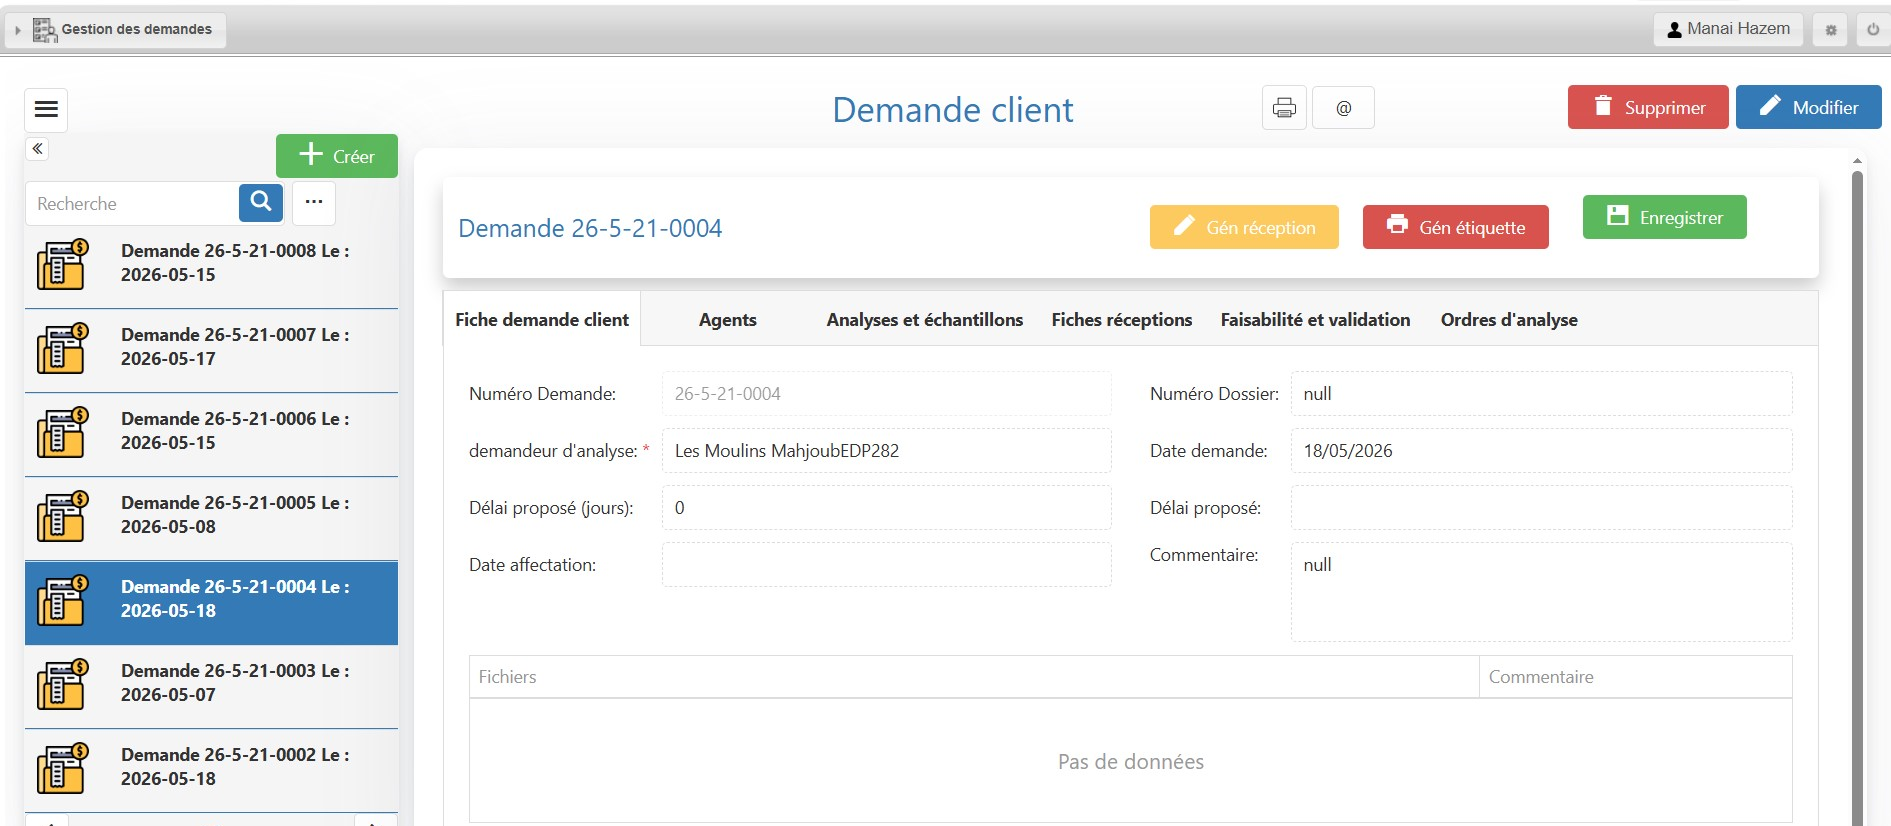
\includegraphics[width=\textwidth]{lims-demande-client.png}
  \caption{Module de gestion des demandes du LIMS.}
  \label{fig:demandes}
\end{figure}

\begin{figure}[H]
  \centering
  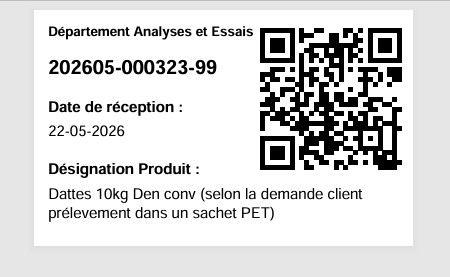
\includegraphics[width=0.5\textwidth]{etiquette-qr-echantillon.png}
  \caption{Étiquette d'échantillon avec code QR générée par le module de gestion des demandes.}
  \label{fig:qr-echantillon}
\end{figure}

Par rapport à l'ancienne étiquette (figure~\ref{fig:codebarre}), la nouvelle étiquette affiche la désignation complète du produit et se lit dans toutes les orientations. Le code \ac{QR} est pour l'instant limité au module de gestion des demandes ; les autres modules conservent le code-barres.

\subsection{Portail client}

Le portail client du \ac{CTAA} (figure~\ref{fig:portail}) complète le \ac{LIMS}. Il permet aux clients de déposer leurs demandes d'analyses, de consulter leurs devis et d'accéder à leurs rapports en ligne, ce qui répond au problème des déplacements identifié lors de l'analyse de l'existant.

\begin{figure}[H]
  \centering
  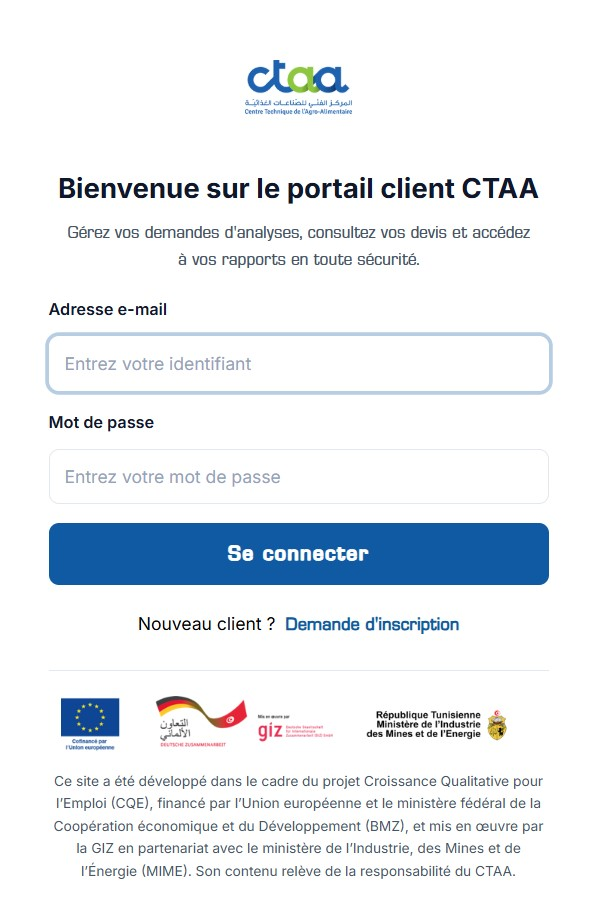
\includegraphics[width=0.45\textwidth]{portail-client-ctaa.jpg}
  \caption{Page de connexion du portail client du CTAA.}
  \label{fig:portail}
\end{figure}

%-------------------------------------------------------------
\section{Réalisation du module de traçabilité}
\label{sec:module-tracabilite}
%-------------------------------------------------------------

\subsection{Interface d'accueil}

L'interface du module (figure~\ref{fig:trace-accueil}) propose deux cases à cocher pour choisir le mode de recherche, « Code à barre » ou « Numéro de série », et un champ unique qui reçoit la lecture de la douchette ou une saisie manuelle.

\begin{figure}[H]
  \centering
  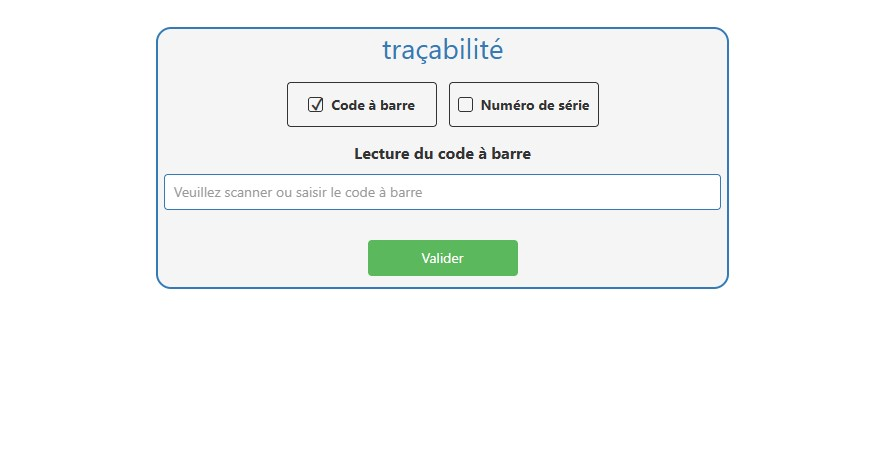
\includegraphics[width=0.75\textwidth]{trace-accueil.jpg}
  \caption{Interface d'accueil du module de traçabilité.}
  \label{fig:trace-accueil}
\end{figure}

\subsection{Traçabilité par code}

En mode « Code à barre », la lecture d'un code de préparation affiche le tableau de traçabilité correspondant : produit, emballage, numéro d'étiquette, lots utilisés, magasin, fournisseur et dates (figure~\ref{fig:trace-code}). Le code lu dans cet exemple est celui décomposé au tableau~\ref{tab:exemple-code}.

\begin{figure}[H]
  \centering
  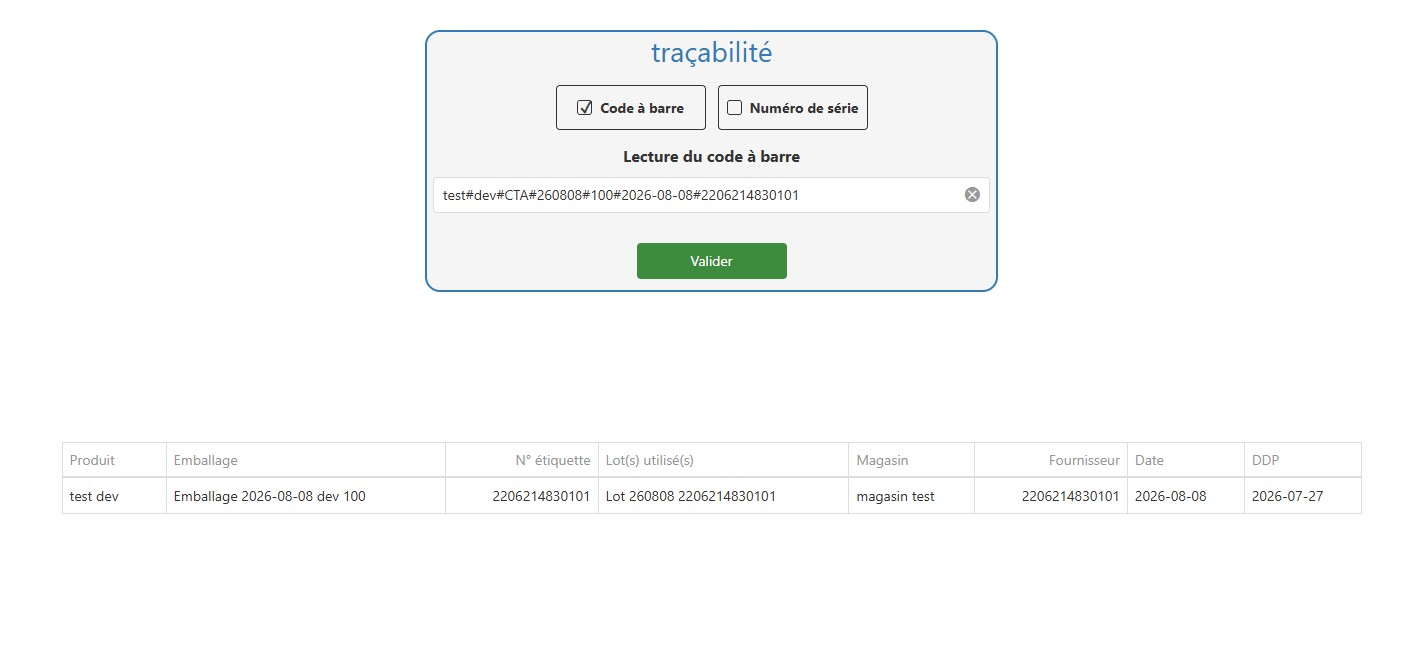
\includegraphics[width=\textwidth]{trace-code-barres.jpg}
  \caption{Traçabilité d'une préparation à partir de son code.}
  \label{fig:trace-code}
\end{figure}

\subsection{Traçabilité par numéro de série}

En mode « Numéro de série », la saisie du numéro de lot \texttt{CS07251350} affiche toutes les lignes de réception qui le concernent : numéro de réception, article, quantités demandée et reçue, \ac{DLC} et utilisateur ayant enregistré la réception (figure~\ref{fig:trace-serie}). Ce résultat est produit par la requête du listing~\ref{lst:requete-serie}, dont la figure~\ref{fig:requete-sql} montre la mise au point dans phpPgAdmin.

\begin{figure}[H]
  \centering
  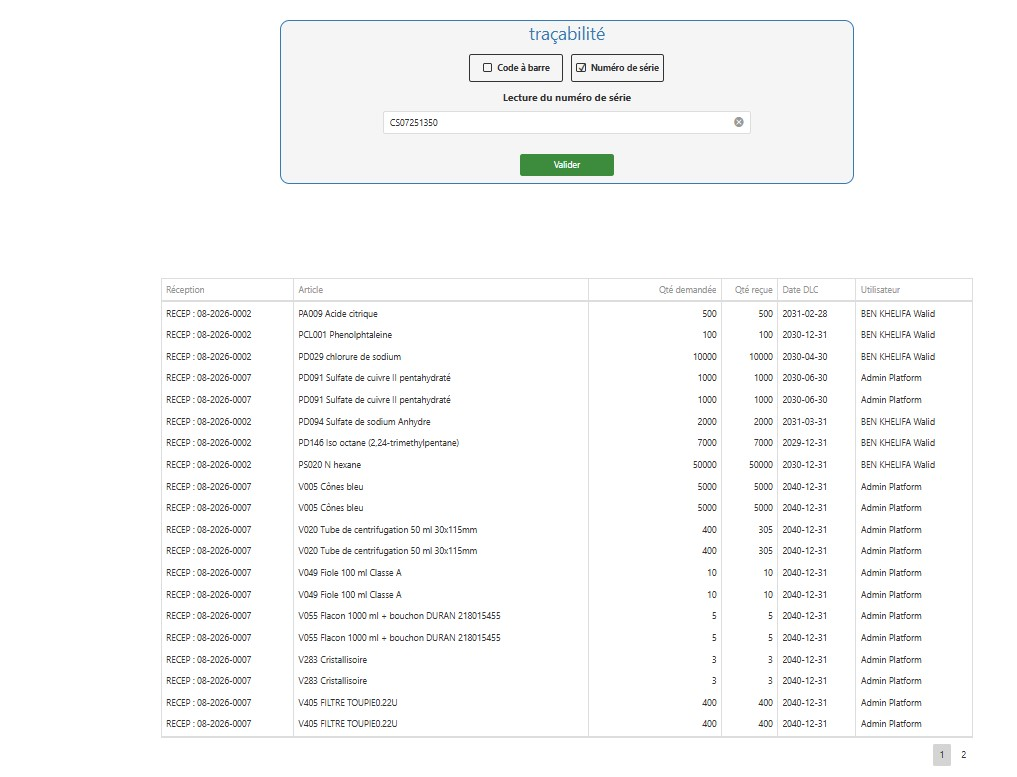
\includegraphics[width=\textwidth]{trace-num-serie.jpg}
  \caption{Traçabilité des réceptions à partir d'un numéro de série.}
  \label{fig:trace-serie}
\end{figure}

\begin{figure}[H]
  \centering
  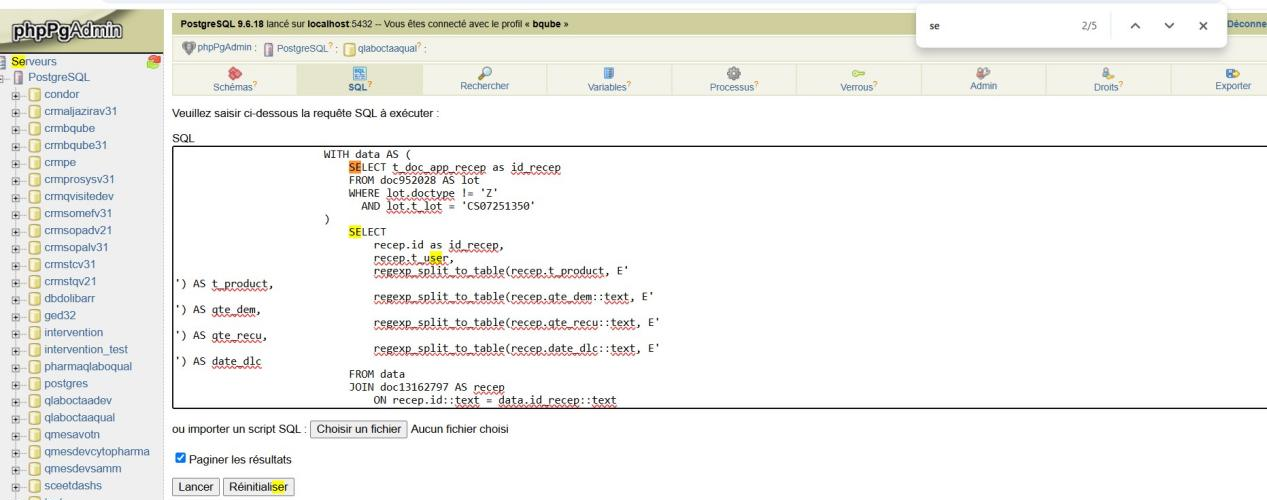
\includegraphics[width=\textwidth]{requete-sql-tracabilite.png}
  \caption{Mise au point de la requête de traçabilité dans phpPgAdmin.}
  \label{fig:requete-sql}
\end{figure}

\subsection{Gestion des erreurs}

Lorsque le code lu ne respecte aucune structure connue ou ne correspond à aucun élément de la base, le module affiche un message explicite invitant l'utilisateur à vérifier la valeur (figure~\ref{fig:trace-erreur}). L'utilisateur peut alors relancer la lecture sans quitter la page.

\begin{figure}[H]
  \centering
  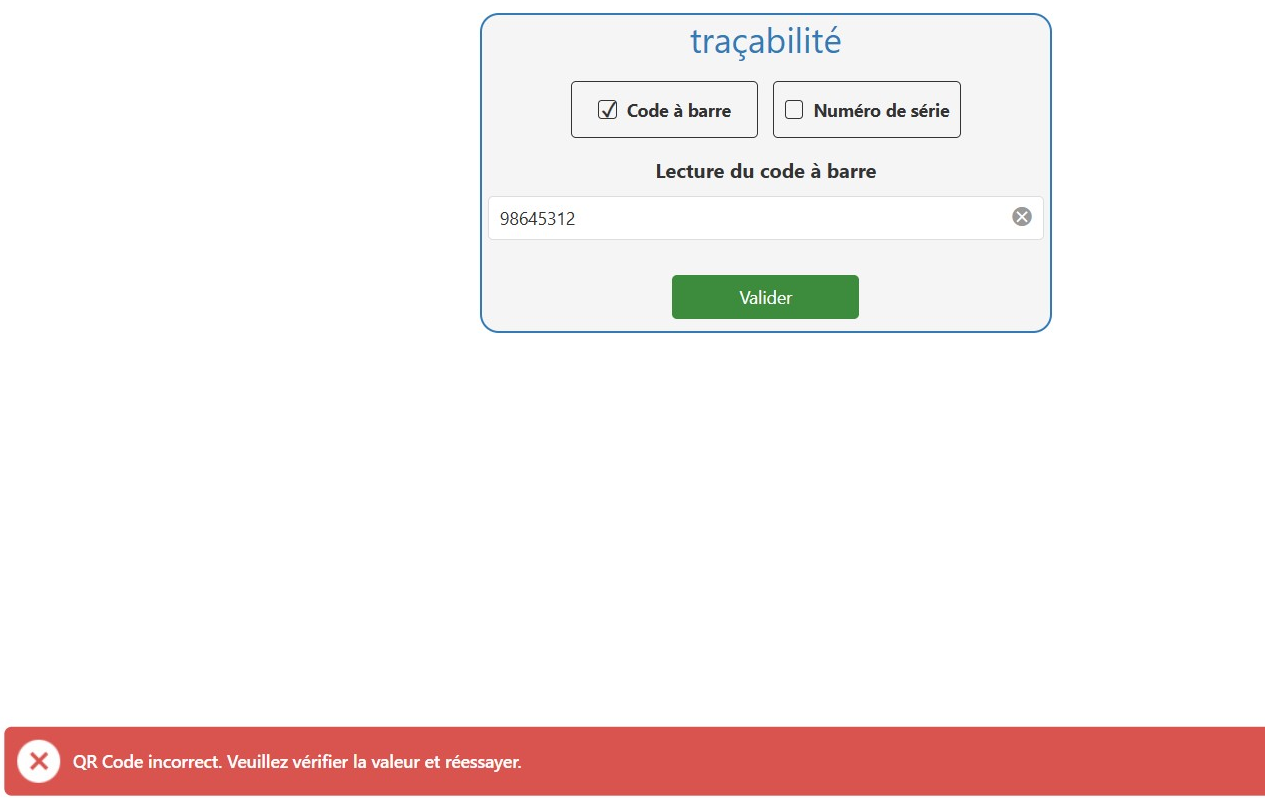
\includegraphics[width=0.85\textwidth]{trace-erreur.png}
  \caption{Message d'erreur affiché pour un code incorrect.}
  \label{fig:trace-erreur}
\end{figure}

\subsection{Extrait du code back-end}

La figure~\ref{fig:code-php} présente un extrait de la fonction \texttt{getDataTabLot} du back-end. On y retrouve les choix de conception décrits au chapitre~\ref{chap:conception} : résolution des familles de documents par leur nom (\texttt{getIdFromName}), lecture des paramètres dans \texttt{config.ini}, connexion à PostgreSQL, puis construction progressive de la clause de filtrage selon les critères reçus (numéro, composant, dates de début et de fin).

\begin{figure}[H]
  \centering
  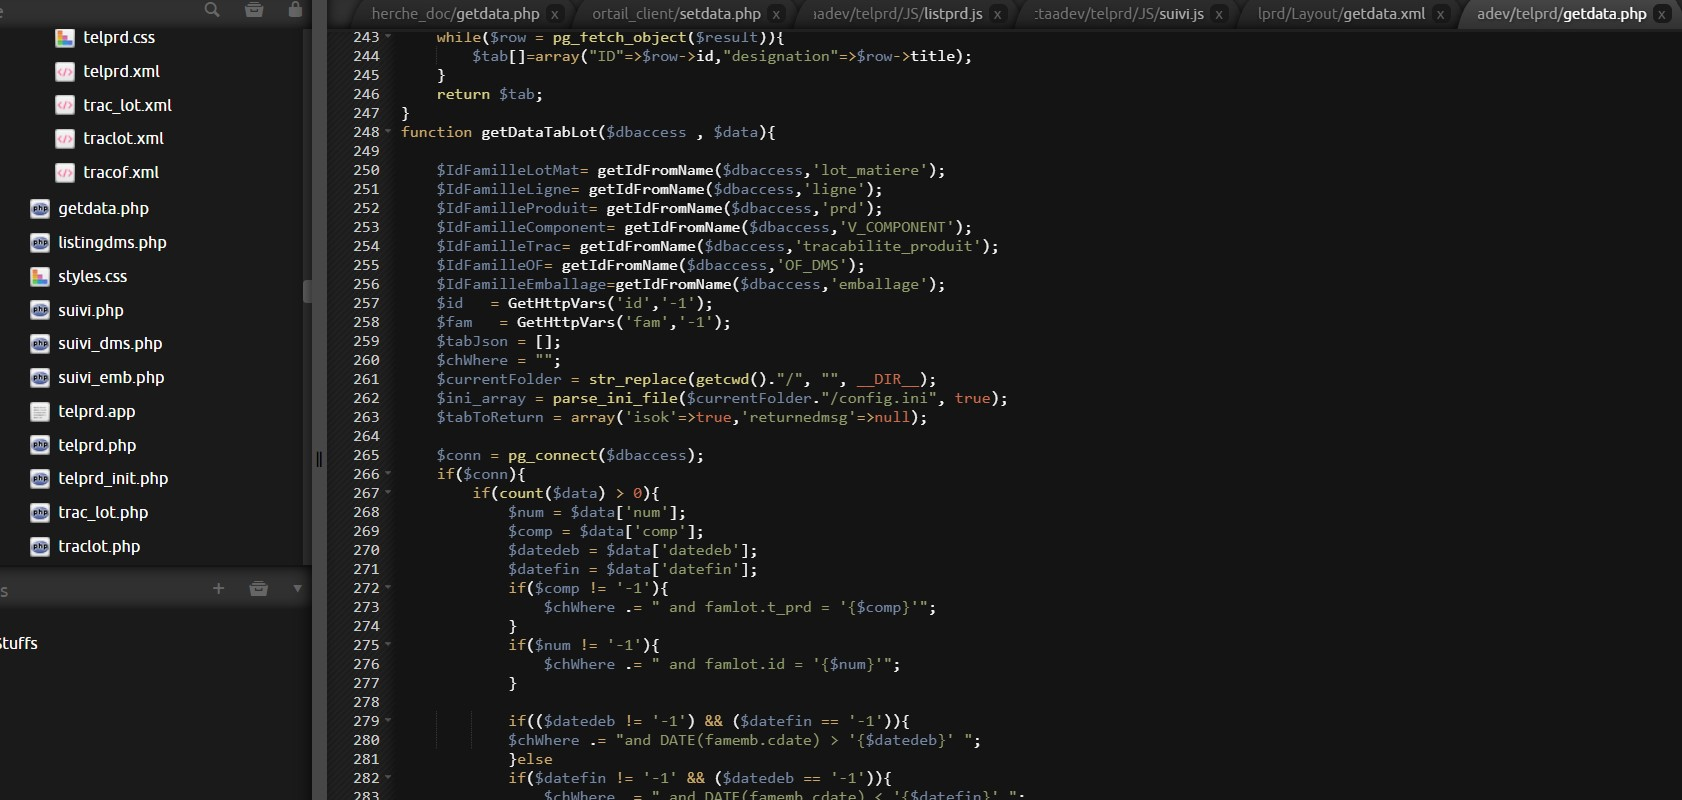
\includegraphics[width=\textwidth]{code-backend-php.png}
  \caption{Extrait du code PHP du back-end du module de traçabilité.}
  \label{fig:code-php}
\end{figure}

%-------------------------------------------------------------
\section{Tests et validation}
%-------------------------------------------------------------

Conformément au cycle en V, chaque fonctionnalité a été vérifiée par rapport aux besoins exprimés au chapitre~\ref{chap:analyse-besoins}. Le tableau~\ref{tab:tests-ctaa} présente les scénarios de test et leurs résultats. Les anomalies relevées lors d'une première série de tests ont été corrigées, puis l'ensemble des scénarios a été rejoué.

% À VÉRIFIER : compléter ou ajuster selon les tests réellement menés.
\begin{table}[H]
\centering
\renewcommand{\arraystretch}{1.25}
\begin{tabularx}{\textwidth}{|c|Y|Y|c|}
\hline
\enteteligne \entete{N°} & \entete{Scénario} & \entete{Résultat attendu} & \entete{Résultat} \\ \hline
T1 & Connexion avec chaque profil d'utilisateur & Accès limité aux fonctionnalités du rôle & Conforme \\ \hline
T2 & Création d'une demande et association des analyses d'un produit & Analyses du pack rattachées automatiquement & Conforme \\ \hline
T3 & Impression d'une étiquette puis lecture de son code QR & Identifiant lu correctement par la douchette & Conforme \\ \hline
T4 & Lecture d'un code de préparation valide (BF1) & Tableau de traçabilité de la préparation & Conforme \\ \hline
T5 & Saisie d'un numéro de série existant (BF2) & Liste des réceptions du lot & Conforme \\ \hline
T6 & Saisie d'un code mal formé (BF4) & Message « code incorrect » & Conforme \\ \hline
T7 & Code bien formé mais absent de la base (BF4) & Message d'erreur, aucune donnée affichée & Conforme \\ \hline
T8 & Comparaison des données affichées avec la base (phpPgAdmin) & Données identiques & Conforme \\ \hline
T9 & Consultation d'un historique incomplet & Affichage des seules opérations existantes, sans erreur & Conforme \\ \hline
\end{tabularx}
\caption{Scénarios de test du LIMS et du module de traçabilité.}
\label{tab:tests-ctaa}
\end{table}

%-------------------------------------------------------------
\section{Formation et accompagnement des utilisateurs}
%-------------------------------------------------------------

\subsection{Enjeux et objectifs}

La réussite d'un \ac{LIMS} ne dépend pas seulement de son paramétrage : elle repose aussi sur son appropriation par les utilisateurs. Un outil bien configuré mais mal maîtrisé reste sous-utilisé, et les anciennes habitudes (papier, fichiers Excel) risquent de revenir. Une part importante de la mission a donc été consacrée à la formation et à l'accompagnement du personnel du \ac{CTAA}, avec quatre objectifs :
\begin{itemize}
    \item rendre chaque utilisateur autonome sur les fonctionnalités liées à son rôle ;
    \item faire comprendre le passage d'un fonctionnement papier à un fonctionnement numérique et centralisé ;
    \item réduire les erreurs d'utilisation pendant les premières semaines ;
    \item recueillir les retours du terrain pour ajuster le système.
\end{itemize}

\subsection{Démarche suivie}

Les contenus ont été adaptés à chaque profil (tableau~\ref{tab:formation-profils}), et l'accompagnement s'est déroulé en quatre temps :
\begin{enumerate}
    \item \textbf{Préparation} : définition du contenu de chaque session et préparation d'exemples tirés des cas réels du laboratoire.
    \item \textbf{Formation fonctionnelle} : animation des sessions, avec un niveau de détail adapté au profil des participants.
    \item \textbf{Accompagnement sur le terrain} : assistance en temps réel des utilisateurs travaillant sur le \ac{LIMS}, notamment pour l'identification par code \ac{QR}.
    \item \textbf{Recueil des retours} : les remarques des utilisateurs ont révélé des écarts entre les processus prévus et les pratiques réelles, et ont servi à ajuster le paramétrage.
\end{enumerate}

\begin{table}[H]
\centering
\renewcommand{\arraystretch}{1.25}
\begin{tabularx}{\textwidth}{|p{3.1cm}|Y|Y|}
\hline
\enteteligne \entete{Profil} & \entete{Contenu et modalités} & \entete{Compétences acquises} \\ \hline
Administrateur & Session technique et accompagnement au paramétrage & Gestion des comptes, des rôles et des droits d'accès \\ \hline
Technicien de laboratoire & Sessions collectives et assistance sur le poste de travail & Enregistrement des échantillons, saisie des résultats, lecture des codes, consultation de la traçabilité \\ \hline
Responsable qualité & Session fonctionnelle et suivi en situation réelle & Suivi des analyses, de la traçabilité, des habilitations et des équipements \\ \hline
Service administratif & Session fonctionnelle courte & Consultation des rapports et suivi des demandes \\ \hline
\end{tabularx}
\caption{Formation des utilisateurs par profil.}
\label{tab:formation-profils}
\end{table}

\subsection{Difficultés rencontrées et solutions apportées}

Le passage au numérique a soulevé plusieurs difficultés :
\begin{itemize}
    \item \textbf{la résistance au changement} : certains utilisateurs étaient attachés aux supports papier ; nous avons mis en avant les bénéfices concrets pour leur travail (moins de ressaisies, recherche plus rapide) ;
    \item \textbf{des niveaux d'aisance informatique différents} : l'accompagnement individuel sur le poste de travail a complété les sessions collectives ;
    \item \textbf{des écarts entre le processus théorique et la pratique} : les retours du terrain ont conduit à des ajustements du paramétrage.
\end{itemize}

Au terme de cette phase, le \ac{LIMS} est intégré aux pratiques quotidiennes du laboratoire, et les utilisateurs perçoivent ses gains concrets : moins de ressaisies et un accès plus rapide à l'information.

%-------------------------------------------------------------
\section{Réalisation du module d'acquisition (Pharmaghreb)}
%-------------------------------------------------------------

\subsection{Étude de connectivité des équipements}

Avant de réaliser le module, nous avons étudié dix équipements du laboratoire de contrôle de Pharmaghreb : interfaces disponibles, protocoles supportés et tests de communication. Le tableau~\ref{tab:etude-equipements} présente les résultats. Il montre que les équipements récents peuvent être interrogés directement par Ethernet, alors que les autres ne disposent que d'une liaison \ac{RS-232}, d'où l'intérêt d'un module d'acquisition.

\begin{table}[H]
\centering
\small
\renewcommand{\arraystretch}{1.25}
\begin{tabularx}{\textwidth}{|p{3.9cm}|p{2.5cm}|Y|}
\hline
\enteteligne \entete{Équipement} & \entete{État} & \entete{Résultat et mode de communication} \\ \hline
Balance Mettler Toledo XPR205 & Communication testée & Ethernet et protocole MT-SICS \\ \hline
Balance Mettler Toledo XSR205 & Communication testée & Ethernet et protocole MT-SICS ; RS-232 et MT-SICS via le module d'acquisition développé \\ \hline
pH-mètre Mettler Toledo SevenExcellence & Communication testée & Ethernet, TCP/IP, via le service de communication Mettler (messages XML) \\ \hline
Titrateur volumétrique compact Karl Fischer V30 & Communication testée & Communication possible uniquement avec le logiciel Mettler LabX \\ \hline
Polarimètre Bellingham + Stanley ADP450 & Communication testée & Ethernet et protocole FTP pour le téléchargement des résultats \\ \hline
Spectromètre L1600300 (logiciel Spectrum) & Communication testée & Liaison Ethernet établie, sans réponse du logiciel Spectrum ; en attente du fournisseur \\ \hline
pH-mètre Mettler Toledo S230 & En attente d'un module ESP32 & RS-232 ou adaptateur USB/RS-232 (à tester) \\ \hline
pH-mètre Mettler Toledo SevenMulti S47 & En attente d'un module ESP32 & Second port RS-232, désactivé selon la documentation (à tester) \\ \hline
Appareil de point de fusion BUCHI M-565 & En attente d'un module ESP32 & RS-232 ou adaptateur USB/RS-232 (à tester) \\ \hline
\end{tabularx}
\caption{Résultats de l'étude de connectivité des équipements de Pharmaghreb.}
\label{tab:etude-equipements}
\end{table}

\subsection{Réalisation du prototype}

Le prototype a été assemblé selon le schéma de câblage de la figure~\ref{fig:cablage}, puis le programme embarqué a été développé selon l'organigramme de la figure~\ref{fig:organigramme}. La balance Mettler Toledo XSR205 a été retenue comme équipement de validation, car elle peut être interrogée à la fois par Ethernet et par \ac{RS-232} : cela permet de comparer les mesures obtenues par les deux voies.

\subsection{Tests du prototype}

Le tableau~\ref{tab:tests-prototype} présente les tests réalisés sur le prototype. Tous les scénarios sont conformes : le module est \textbf{complet et fonctionnel}, et il attend son déploiement sur site.

% À VÉRIFIER : ajuster selon les tests réellement menés.
\begin{table}[H]
\centering
\renewcommand{\arraystretch}{1.25}
\begin{tabularx}{\textwidth}{|c|Y|Y|c|}
\hline
\enteteligne \entete{N°} & \entete{Scénario} & \entete{Résultat attendu} & \entete{Résultat} \\ \hline
P1 & Envoi de la commande \texttt{S} à la balance XSR205 & Trame reçue et valeur décodée & Conforme \\ \hline
P2 & Pesée en cours de stabilisation & Valeur instable non enregistrée & Conforme \\ \hline
P3 & Présentation d'un badge NFC & Identifiant lu et associé aux mesures & Conforme \\ \hline
P4 & Premier démarrage sans réseau connu & Ouverture du point d'accès de configuration & Conforme \\ \hline
P5 & Connexion au réseau local & Adresse IP affichée sur l'écran LCD & Conforme \\ \hline
P6 & Appui de 5 s sur le bouton & Configuration Wi-Fi effacée & Conforme \\ \hline
P7 & Requête HTTP sur \texttt{/getData} & Dernière mesure renvoyée au format JSON & Conforme \\ \hline
\end{tabularx}
\caption{Scénarios de test du module d'acquisition.}
\label{tab:tests-prototype}
\end{table}

\subsection{État d'avancement}

Le module d'acquisition est réalisé et validé en laboratoire. Les prochaines étapes sont :
\begin{itemize}
    \item le déploiement du module sur le poste de pesée et sa validation en conditions réelles ;
    \item l'intégration des mesures au système d'information de Pharmaghreb, puis au \ac{LIMS} ;
    \item la connexion des équipements en attente, à l'aide de modules ESP32 ;
    \item le développement d'une interface de supervision centralisée.
\end{itemize}

%-------------------------------------------------------------
\section*{Conclusion}
\addcontentsline{toc}{section}{Conclusion}
%-------------------------------------------------------------

Ce chapitre a présenté la réalisation des deux solutions. Au \ac{CTAA}, le \ac{LIMS} a été paramétré et mis en service, l'étiquetage des échantillons par code \ac{QR} a été mis en place dans le module de gestion des demandes, et le module de traçabilité a été développé, testé et adopté grâce à la formation des utilisateurs. Chez Pharmaghreb, l'étude de connectivité de dix équipements a guidé la réalisation d'un module d'acquisition complet et testé, qui attend son déploiement.

\chapter*{Conclusion générale et perspectives}
\addcontentsline{toc}{chapter}{Conclusion générale et perspectives}
\markboth{Conclusion générale et perspectives}{}

Ce projet de fin d'études, réalisé au sein de BQube ITs, avait pour objectif de contribuer à la digitalisation des processus analytiques de laboratoire, de la gestion des échantillons jusqu'aux équipements connectés. Il a été mené sur deux terrains complémentaires, qui couvrent les deux niveaux de la transformation numérique : le système d'information et les équipements.

Au \textbf{Centre Technique de l'Agro-Alimentaire}, nous avons participé au paramétrage et à la mise en service d'un \ac{LIMS} : création des utilisateurs et de leurs droits, configuration des produits et des packs d'analyses, étiquetage des échantillons par code \ac{QR} dans le module de gestion des demandes. Nous avons ensuite conçu et développé un module de traçabilité, en \ac{PHP}, JavaScript et PostgreSQL, qui reconstitue l'historique d'une préparation ou d'une réception à partir de la lecture d'un code ou de la saisie d'un numéro de série. La formation et l'accompagnement des utilisateurs ont permis d'ancrer ces outils dans les pratiques quotidiennes du laboratoire. L'estimation des gains montre un investissement récupéré en 13 à 15 mois et un \ac{ROI} supérieur à 130\,\% sur trois ans.

Aux \textbf{Laboratoires Pharmaghreb}, nous avons étudié la connectivité de dix équipements de laboratoire et identifié, pour chacun, la voie de communication la plus adaptée : Ethernet avec les protocoles \ac{MT-SICS}, \ac{TCP}/\ac{IP} ou \ac{FTP}, ou liaison \ac{RS-232}. Pour les équipements qui ne disposent que d'une liaison série, nous avons conçu, réalisé et testé un module d'acquisition à base d'ESP8266, qui récupère les mesures stables d'une balance, les associe à l'opérateur identifié par badge \ac{NFC} et les met à disposition par \ac{Wi-Fi}. Ce prototype est fonctionnel et attend son déploiement.

Sur le plan personnel, ce projet a constitué une expérience particulièrement enrichissante. Il nous a permis de consolider nos connaissances en Industrie~4.0 et en Internet industriel des objets, de mettre en pratique le développement web et l'électronique embarquée, et de découvrir les exigences d'un déploiement réel : écoute des utilisateurs, conduite du changement et respect des contraintes réglementaires des laboratoires.

\section*{Perspectives}

Plusieurs évolutions peuvent prolonger ce travail :
\begin{itemize}
    \item \textbf{généraliser le code \ac{QR}} aux autres modules du \ac{LIMS} (réceptions, préparations, stocks), afin d'uniformiser l'identification ;
    \item \textbf{renforcer le module de traçabilité} par des requêtes paramétrées côté serveur, des tableaux de bord et un système d'alertes ;
    \item \textbf{déployer le module d'acquisition} sur site et intégrer ses mesures au \ac{LIMS}, pour assurer une continuité numérique de l'équipement jusqu'au rapport d'analyse ;
    \item \textbf{connecter les autres équipements} étudiés, à l'aide de modules ESP32 pour les liaisons série et des interfaces Ethernet pour les équipements récents ;
    \item \textbf{mettre en place une supervision centralisée} de l'état et des performances des équipements ;
    \item \textbf{exploiter les données collectées} par des outils d'analyse et d'intelligence artificielle, afin de détecter les anomalies et d'évoluer vers la maintenance prédictive.
\end{itemize}

À plus long terme, ces évolutions conduiraient à un laboratoire dans lequel les équipements ne sont plus des systèmes isolés, mais des sources de données connectées au système d'information, au service de la qualité, de la traçabilité et de la prise de décision.


\cleardoublepage
\phantomsection
\addcontentsline{toc}{chapter}{Bibliographie}
\renewcommand{\bibname}{Bibliographie}
\bibliographystyle{apalike}
\bibliography{references}

\appendix
\chapter{Méthode d'estimation des gains économiques}
\label{annexe:gains}

Cette annexe détaille la méthode utilisée pour estimer les gains économiques présentés au chapitre~\ref{chap:cadre-general} (tableaux~\ref{tab:gains-ctaa} et~\ref{tab:gains-pharmaghreb}), les hypothèses retenues et la sensibilité des résultats.

% IMPORTANT : les hypothèses ci-dessous reproduisent les montants estimés. Elles doivent
% être confirmées (ou remplacées) par des valeurs mesurées sur le terrain.

\section{Principe de la méthode}

Le gain annuel d'une solution de digitalisation provient essentiellement du temps libéré pour le personnel, auquel s'ajoutent des économies directes (papier, consommables). Pour chaque source de gain $i$, on estime :
\[
G_i = N_i \times \Delta t_i \times C_h
\qquad\text{et}\qquad
G_{\text{an}} = \sum_i G_i + E_{\text{directes}}
\]
où $N_i$ est le nombre annuel d'opérations concernées, $\Delta t_i$ le temps gagné par opération (en heures), $C_h$ le coût horaire chargé du personnel et $E_{\text{directes}}$ les économies directes. La méthode se déroule en six étapes :
\begin{enumerate}
    \item \textbf{identifier les sources de gain} à partir de l'analyse de l'existant et des sept Muda (saisie, recherche, archivage, erreurs, consommables, disponibilité des équipements) ;
    \item \textbf{quantifier les volumes} $N_i$ à partir des données d'activité (demandes par jour, échantillons par demande, mesures par jour) et d'un nombre de 250 jours ouvrés par an ;
    \item \textbf{mesurer le temps gagné} $\Delta t_i$ par chronométrage d'une vingtaine d'opérations avant et après la digitalisation ;
    \item \textbf{valoriser} ce temps au coût horaire chargé $C_h$ (salaire brut et charges patronales, divisés par le nombre d'heures travaillées) ;
    \item \textbf{encadrer l'incertitude} par deux scénarios : un scénario prudent (volumes bas) et un scénario optimiste (volumes hauts) ;
    \item \textbf{calculer les indicateurs} (délai de récupération et \ac{ROI}) et \textbf{tester leur sensibilité} aux hypothèses les plus incertaines.
\end{enumerate}

\section{Application au CTAA}

Le tableau~\ref{tab:hyp-ctaa} présente les hypothèses retenues pour le \ac{CTAA}, avec un coût horaire chargé de 15~\ac{TND}/h et 250 jours ouvrés par an. Les volumes s'appuient sur l'analyse de l'existant : 10 à 20 demandes par jour, soit en moyenne une soixantaine d'échantillons.

\begin{table}[H]
\centering
\small
\renewcommand{\arraystretch}{1.25}
\begin{tabularx}{\textwidth}{|p{2.9cm}|Y|r|r|}
\hline
\enteteligne \entete{Source de gain} & \entete{Hypothèse de calcul} & \entete{Prudent} & \entete{Optimiste} \\ \hline
Traitement des demandes & 15 (prudent) ou 20 (optimiste) demandes/jour $\times$ 250 j $\times$ 20 min gagnées $\times$ 15 TND/h & 18\,750 & 25\,000 \\ \hline
Recherche des échantillons & 60 échantillons/jour $\times$ 250 j $\times$ 6 min gagnées $\times$ 15 TND/h & 22\,500 & 22\,500 \\ \hline
Archivage & 200 h/an de classement évitées $\times$ 15 TND/h & 3\,000 & 3\,000 \\ \hline
Réduction des erreurs & 100 h/an de détection et de correction évitées $\times$ 15 TND/h & 1\,500 & 1\,500 \\ \hline
Papier & Économie directe d'environ 100 TND/mois $\times$ 12 & 1\,200 & 1\,200 \\ \hline
\rowcolor{bleuclair} \multicolumn{2}{|l|}{\textbf{Total (TND/an)}} & \textbf{46\,950} & \textbf{53\,200} \\ \hline
\end{tabularx}
\caption{Hypothèses de calcul des gains annuels au CTAA.}
\label{tab:hyp-ctaa}
\end{table}

\section{Application à Pharmaghreb}

Le tableau~\ref{tab:hyp-pharmaghreb} présente les hypothèses retenues pour Pharmaghreb, avec un coût horaire chargé de 20~\ac{TND}/h, plus élevé que dans le secteur public, et 250 jours ouvrés par an.

\begin{table}[H]
\centering
\small
\renewcommand{\arraystretch}{1.25}
\begin{tabularx}{\textwidth}{|p{2.9cm}|Y|r|r|}
\hline
\enteteligne \entete{Source de gain} & \entete{Hypothèse de calcul} & \entete{Prudent} & \entete{Optimiste} \\ \hline
Saisies manuelles & 144 ou 180 mesures/jour $\times$ 250 j $\times$ 1 min de saisie et de vérification $\times$ 20 TND/h & 12\,000 & 15\,000 \\ \hline
Temps de collecte & 2 h ou 2,5 h/jour de relevés et de regroupement $\times$ 250 j $\times$ 20 TND/h & 10\,000 & 12\,500 \\ \hline
Disponibilité des équipements & 375 h/an d'immobilisation évitées $\times$ 20 TND/h & 7\,500 & 7\,500 \\ \hline
Centralisation des données & 1 h/jour de consolidation évitée $\times$ 250 j $\times$ 20 TND/h & 5\,000 & 5\,000 \\ \hline
Réduction des erreurs & 100 h/an d'investigations et de reprises évitées $\times$ 20 TND/h & 2\,000 & 2\,000 \\ \hline
\rowcolor{bleuclair} \multicolumn{2}{|l|}{\textbf{Total (TND/an)}} & \textbf{36\,500} & \textbf{42\,000} \\ \hline
\end{tabularx}
\caption{Hypothèses de calcul des gains annuels chez Pharmaghreb.}
\label{tab:hyp-pharmaghreb}
\end{table}

Le coût de déploiement n'étant pas encore arrêté, le \ac{ROI} réel ne peut pas encore être calculé. On peut en revanche déterminer le \textbf{seuil de rentabilité} : le \ac{ROI} sur trois ans reste positif tant que l'investissement $I_0$ ne dépasse pas trois années de gains, soit 109\,500~TND dans le scénario prudent et 126\,000~TND dans le scénario optimiste. De même, l'investissement est récupéré en moins d'un an s'il reste inférieur au gain annuel, soit 36\,500~TND dans le scénario prudent.

\section{Analyse de sensibilité}

Le calcul du chapitre~\ref{chap:cadre-general} suppose qu'aucun coût récurrent ne s'ajoute à l'investissement initial. Le tableau~\ref{tab:sensibilite} montre l'effet, pour le \ac{CTAA}, d'un coût récurrent annuel $M$ (maintenance, hébergement) de 10\,000~TND, puis d'une baisse de 20\,\% des gains. Le \ac{ROI} devient alors :
\[
\text{ROI}_{3\,\text{ans}} = \frac{3\,(G_{\text{an}} - M) - I_0}{I_0} \times 100
\]

\begin{table}[H]
\centering
\renewcommand{\arraystretch}{1.25}
\begin{tabular}{|l|r|r|r|r|}
\hline
\enteteligne & \multicolumn{2}{c|}{\entete{Délai (mois)}} & \multicolumn{2}{c|}{\entete{ROI sur 3 ans}} \\ \hline
\rowcolor{bleuclair} \textbf{Cas} & \textbf{Prudent} & \textbf{Optimiste} & \textbf{Prudent} & \textbf{Optimiste} \\ \hline
Cas de base & 15,3 & 13,5 & 134,75\,\% & 166\,\% \\ \hline
Coût récurrent de 10\,000 TND/an & 19,5 & 16,7 & 84,75\,\% & 116\,\% \\ \hline
Gains réduits de 20\,\% & 19,2 & 16,9 & 87,8\,\% & 112,8\,\% \\ \hline
\end{tabular}
\caption{Sensibilité du délai de récupération et du ROI au CTAA.}
\label{tab:sensibilite}
\end{table}

Même dans ces cas défavorables, l'investissement est récupéré en moins de deux ans et le \ac{ROI} sur trois ans reste largement positif, ce qui confirme la robustesse de la conclusion.


\cleardoublepage
\thispagestyle{empty}
\pagestyle{empty}

\noindent{\color{bleu}\rule{\textwidth}{0.6pt}}\\[0.2cm]
\noindent{\large\textbf{Résumé}}\\[0.2cm]
Ce projet de fin d'études, réalisé au sein de BQube ITs, porte sur la transformation numérique des processus analytiques de laboratoire. Au Centre Technique de l'Agro-Alimentaire (CTAA), nous avons participé au paramétrage et à la mise en service d'un système de gestion des informations de laboratoire (LIMS), mis en place l'étiquetage des échantillons par code QR et formé les utilisateurs. Nous avons également conçu et développé, en PHP, JavaScript et PostgreSQL, un module de traçabilité qui reconstitue l'historique des opérations à partir de la lecture d'un code ou d'un numéro de série. Aux Laboratoires Pharmaghreb, nous avons étudié la connectivité de dix équipements de laboratoire, puis conçu, réalisé et testé un prototype d'acquisition à base d'ESP8266 qui récupère les mesures d'une balance par liaison RS-232 selon le protocole MT-SICS, identifie l'opérateur par badge NFC et transmet les données par Wi-Fi.\\[0.2cm]
\noindent\textbf{Mots clés :} LIMS, Industrie 4.0, traçabilité, code QR, IIoT, ESP8266, RS-232, ISO/CEI 17025.\\
\noindent{\color{bleu}\rule{\textwidth}{0.6pt}}

\vspace{1.5cm}

\noindent{\color{bleu}\rule{\textwidth}{0.6pt}}\\[0.2cm]
\noindent{\large\textbf{Abstract}}\\[0.2cm]
\begin{otherlanguage}{english}
This graduation project, carried out at BQube ITs, deals with the digital transformation of laboratory analytical processes. At the Technical Center for Agri-Food (CTAA), we took part in configuring and commissioning a Laboratory Information Management System (LIMS), set up QR code labelling of samples and trained the users. We also designed and developed, using PHP, JavaScript and PostgreSQL, a traceability module that reconstructs the history of operations from a scanned code or a serial number. At Pharmaghreb Laboratories, we studied the connectivity of ten laboratory instruments, then designed, built and tested an ESP8266-based acquisition prototype that retrieves the measurements of a balance over an RS-232 link using the MT-SICS protocol, identifies the operator with an NFC badge and transmits the data over Wi-Fi.\\[0.2cm]
\noindent\textbf{Keywords:} LIMS, Industry 4.0, traceability, QR code, IIoT, ESP8266, RS-232, ISO/IEC 17025.
\end{otherlanguage}\\
\noindent{\color{bleu}\rule{\textwidth}{0.6pt}}


\end{document}
